% !TeX spellcheck = es_ES
% !TEX encoding = UTF-8 Unicode
\documentclass[t, compress, spanish, aspectratio=169]{beamer}
%\documentclass[handout]{beamer}    % for the handout

\usetheme[progressbar=frametitle]{metropolis}

%\usetheme[secheader]{Madrid}
%\usetheme{Frankfurt}
%\usetheme{Warsaw}
%\usetheme{Berlin}
%\usetheme{CambridgeUS}

%\usecolortheme{beaver}     % Fondo Blanco y letras Negras - Titulos en Rojo con fondo gris
%\usecolortheme{dove}       % Para el Handout
%\usecolortheme{seahorse}   % Fondo Blanco y letras Negras - Titulos en Celeste
%\usecolortheme{dolphin}    % Fondo Blanco y letras Negras - Titulos en Celeste
%\usecolortheme{seagull}    % Fondo Blanco y letras Negras - Titulos en Gris
%\usecolortheme{crane}      % Fondo Blanco y letras Negras - Titulos en Amarillo
%\usecolortheme{wolverine}  % Fondo Blanco y Letras negras - Titulos en negro con fondo amarillo
%\usecolortheme{lily}       % Fondo Blanco y letras Negras - Titulos en Azul
%\usecolortheme{fly}        % Fondo Gris y letras Negras - Titulos en Rojo
%\usecolortheme{beetle}     % Fondo Gris y letras Negras - Titulos en blanco
%\usecolortheme{albatross}  % Fondo Azul y letras blancas
%\usecolortheme{orchid}     % Default
%\usecolortheme{rose}       % Default
%\usecolortheme{whale}      % Default

\setbeamertemplate{navigation symbols}{} % Gets rid of navigation symbols
%\setbeamercovered{transparent}

\usepackage{dsfont} % Double stroke fonts for math symbols
% \usepackage[T1]{fontenc}  % Helps with hyphenation for languages with accented characters. Note: Does not work with XeLaTex
% \usepackage[latin1]{inputenc} % Allows to type in latin (accents). Note: Does not work with XeLaTex
% \usefonttheme[onlymath]{serif}  % Changes fonts for math to serif
\usepackage[english]{babel} % Manages differences between languages: hyphenation etc

\usepackage{appendixnumberbeamer} % Does not include backup slides in the number of pages

\usepackage{centernot} % To draw not in math symbols (does not imply)

\usepackage{ragged2e}  % Text alignment
\justifying

\usepackage{graphicx} % Format for graphics: additional options for includefigure
\usepackage{pgf} % Tool for graphics

\usepackage{booktabs} % Format for tables: top, bottom and mid lines
\usepackage[scale=2]{ccicons}
\usepackage{threeparttable} % Format for tables
\usepackage{lscape} % Landscape for tables

% Customized commands
  \newcommand{\vs}{\vskip0pt plus.5fill}
  \newcommand{\SR}{\mathbb{R}}
  \DeclareMathOperator{\plim}{plim}
  \DeclareMathOperator{\Var}{Var}
  \DeclareMathOperator{\Avar}{AVar}
  \DeclareMathOperator{\Cov}{Cov}
  \DeclareMathOperator{\N}{Normal}
  \DeclareMathOperator{\E}{\mathbb{E}}
  \DeclareMathOperator{\LP}{\mathbb{L}}
  \newcommand{\pto}{\stackrel{p}{\longrightarrow}}
  \newcommand{\dto}{\stackrel{d}{\longrightarrow}}
  \newcommand{\adistr}{\stackrel{a}{\sim}}
  \newcommand{\epsi}{\varepsilon}
  \newcommand{\tmle}{\hat \theta_{ML}}
  \newcommand{\tgmm}{\hat \theta_{GMM}}
  \newcommand\independent{\protect\mathpalette{\protect\independenT}{\perp}}
  \def\independenT#1#2{\mathrel{\rlap{$#1#2$}\mkern2mu{#1#2}}}


\title [Estimaci\'on por MCO] {Econometr\'ia I\\
	Modelo Lineal de Regresi\'on: Estimaci\'on por MCO}
\author[de Elejalde]{Ramiro de Elejalde}
\institute [UAH] {Facultad de Econom\'ia y Finanzas \\ Universidad Alberto Hurtado}
\date[\today] {}
\subject{Econometr\'ia}
\begin{document}
	
	%------------------------------------------------------------
	
	\begin{frame}
		\titlepage
	\end{frame}
	
	% --------------------------------------------------- Slide --
	\begin{frame}
		\frametitle{Outline}
		\tableofcontents
		\alert{Referencias}: Cap. 7 de Hansen, cap. 4.1, 4.2 (excepto 4.2.4) y 4.3.1 de Wooldridge, cap. 6 de Stock and Watson, y cap. 3.1.3 y 3.2.2 de Angrist and Pischke.
	\end{frame}
	% --------------------------------------------------- Slide --
	\section[Motivaci\'on: Tama\~no de clase y rendimiento acad\'emico]{Motivaci\'on: Efecto del tama\~no de clase en el rendimiento acad\'emico (California)}
	\begin{frame}
		\frametitle{Efecto del tama\~no de clase en el rendimiento acad\'emico (California)}
		\begin{itemize}
			\item \alert{Pregunta de pol\'itica}: ?`Cu\'al es el efecto de reducir el tama\~no de clase en el rendimiento escolar?
			\item \alert{Datos}: Todos los distritos escolares de escuelas K-6 y K-8 de California ($N=420$)
			\item \alert{Variables}:
			\begin{itemize}
				\item Notas de examen de 5to grado (Stanford-9 achievement test, matem\'atica y lectura), media del distrito (\alert{testscr})
				\item Ratio estudiantes por profesor: n\'umero de estudiantes en el distrito divido por el n\'umero de profesores tiempo completo (\alert{str}).
			\end{itemize}
		\end{itemize}
	\end{frame}
	% --------------------------------------------------- Slide --
	\begin{frame}
		\frametitle{Estad\'isticas descriptivas}
		\begin{table}
			\caption{Resumen de la distribuci\'on de los ratios de estudiantes por profesor y notas en test estandarizados para 5to grado para 420 distritos escolares en California en 1998}
			\centering
			\tiny
			\begin{tabular}{l c c c c c c c}
				\toprule
				&       &            & \multicolumn{5}{c}{Percentil}                    \\
				\cmidrule(r){4-8}                                                       \\
				&       & Desviaci\'on &   10\% &   25\%   &     50\%  &   75\% &  90\%   \\
				& Media & Est\'andar   &        &          & (mediana) &        &         \\
				\midrule
				Estudiantes/profesor      &  19.6 &      1.9   &   17.3 &   18.6   &      19.7 &   20.9 &   21.9  \\
				Nota en test             & 654.2 &     19.1   &  630.4 &  640.0   &     654.5 &  666.7 &  679.1  \\
				\bottomrule
			\end{tabular}
		\end{table}
	\end{frame}
	% --------------------------------------------------- Slide --
	\begin{frame}
		\begin{figure}[h!]
			\caption{Scatter plot de notas versus ratio estudiantes/profesor}
			\centering
			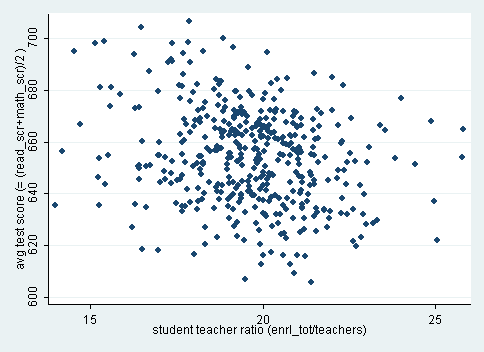
\includegraphics[width=0.7\textwidth]{figures/scatter_student_teacher_scores.png}
		\end{figure}
	\end{frame}
	% --------------------------------------------------- Slide --
	\begin{frame}
		\frametitle{Efecto causal}
		\small
		\begin{itemize}
			\item  []
			\begin{align*}
				testscr_i = \beta_0 + \beta_1 \, str_i + u_i,
			\end{align*}
			donde $u_i$ contiene todos los factores que influyen sobre el rendimiento escolar adem\'as del tama\~no de clase.
			\item  \alert{Efecto causal}: $\beta_1$ mide el efecto causal de aumentar el tama\~no de clase en rendimiento acad\'emico. \\
			Podemos usar $\beta_1$ para responder: ?`Cu\'al es el efecto de cambiar un estudiante de una clase de 22 estudiantes a una clase de 17 estudiantes?
			% Estamos tratando de hacer un ejercicio contrafactual: Aprender sobre la diferencia entre un resultado observado y un resultado potencial no observado.
		\end{itemize}
	\end{frame}
	% --------------------------------------------------- Slide --
	\begin{frame}
		\frametitle{Efecto causal}
		\small
		\begin{itemize}
			\item  []
			\begin{align*}
				testscr_i = \beta_0 + \beta_1 \, str_i + u_i,
			\end{align*}
			donde $u_i$ contiene todos los factores que influyen sobre el rendimiento escolar adem\'as del tama\~no de clase.
			\item  \alert{Efecto causal}: $\beta_1$ mide el efecto causal de aumentar el tama\~no de clase en rendimiento acad\'emico. \\
			\item  Para poder estimar $\beta_1$ necesitamos imponer supuestos sobre $u_i$.
			\item  [] Formalmente: \alert{$\E(u_i|str_i)=0$}.
		\end{itemize}
	\end{frame}

	% --------------------------------------------------- Slide --
	\begin{frame}
		\frametitle{Efecto causal}
		\small
		\begin{itemize}
			\item []
			\begin{align*}
				testscr_i = \beta_0 + \beta_1 \, str_i + u_i,
			\end{align*}
			\item \alert{Efecto causal}: Necesitamos \alert{$\E(u_i|str_i)=0$}.
			\item Intuitivamente: No debe haber diferencias sistem\'aticas en factores que puedan afectar el rendimiento acad\'emico en alumnos que asisten a escuelas con distintos tama\~no de clase.
			\begin{enumerate}
			    \item Buscar \alert{factores que puedan afectar el rendimientos acad\'emico} (adem\'as del tama\~no de clase).
			    \item Intuir si estos \alert{factores difieren seg\'un el tama\~no de clase}.
			\end{enumerate}
		\end{itemize}
	\end{frame}
	% --------------------------------------------------- Slide --
	\begin{frame}
		\frametitle{Efecto causal}
		\small
		\begin{itemize}
			\item []
			\begin{align*}
				testscr_i = \beta_0 + \beta_1 \, str_i + u_i,
			\end{align*}
			\item \alert{Efecto causal}: Necesitamos \alert{$\E(u_i|str_i)=0$}.
			\item Expresa la idea que es imposible observar simult\'aneamente un mismo estudiante en un clase de 17 alumnos y en una clase de 22 alumnos. Sin embargo, podemos comparar los resultados de estudiantes en clases de 17 alumnos y en clases de 22 alumnos. Establece, bajo que condiciones, esta comparaci\'on permite medir el efecto causal buscado.
		\end{itemize}
	\end{frame}
	% --------------------------------------------------- Slide --
	\begin{frame}
		\frametitle{Efecto causal}
		\begin{itemize}
			\item  []
		\begin{align*}
				testscr_i = \beta_0 + \beta_1 \, str_i + u_i
			\end{align*}
			donde $u_i$ contiene todos los factores que influyen sobre el rendimiento escolar adem\'as del tama\~no de clase.
			\item ?`En qu\'e situaciones el supuesto \alert{$\E(u_i|str_i)=0$} puede ser v\'alido?
			\item \alert{Asignaci\'on aleatoria} por tama\~no de clase. ?`Por qu\'e?
			\item [] Ejemplo: El proyecto STAR (Student-Teacher Achievement Ratio) en Tennessee, USA.
		\end{itemize}
	\end{frame}

	% --------------------------------------------------- Slide --
	\begin{frame}
		\frametitle{Efecto causal}
		\begin{itemize}
			\item Si no hay asignaci\'on aleatoria por tama\~no de clase debemos buscar una estrategia alternativa para identificar el efecto causal
			\item Comparamos alumnos con variables \alert{observables} similares (ingreso, educaci\'on de los padres, motivaci\'on, etc.) pero en clases de distinto tama\~no: 
			\alert{asignaci\'on aleatoria condicional en observables}.
			\begin{align*}
				testscr_i = \beta_0 + \beta_1 \, str_i + \gamma' \, x_i + v_i,
			\end{align*}
			%donde $u_i$ contiene todos los factores que influyen sobre el rendimiento escolar adem\'as del tama\~no de clase.
			donde $x_i$ incluye ingreso, educaci\'on de los padres, motivaci\'on, etc.
			\item  Ejemplo: Efecto de veterano de guerra en salarios.
		\end{itemize}
	\end{frame}
	% --------------------------------------------------- Slide --
	\begin{frame}
		\frametitle{Efecto causal}
		\begin{itemize}
			\item  []
			\begin{align*}
				testscr_i = \beta_0 + \beta_1 \, str_i + u_i
			\end{align*}
			donde $\E(u_i|str_i)=0$
			\item \alert{Esperanza condicional}: 
			\begin{align*}
			\E(testscr_i|str_i) = \beta_0 + \beta_1 \, str_i
			\end{align*}
			\item []  \alert{Importante}: El supuesto $\E(u_i|str_i)=0$ nos permite dar una interpretaci\'on causal a la esperanza condicional.
		\end{itemize}
	\end{frame}	
	% --------------------------------------------------- Slide --
	\begin{frame}
		\frametitle{Efecto causal}
		\begin{itemize}
			\item  []
			\begin{align*}
				testscr_i = \beta_0 + \beta_1 \, str_i + u_i
			\end{align*}
			donde $\E(u_i|str_i)=0$
			\item  \alert{Modelo de regresi\'on lineal}: 
			\begin{align*}
			testscr_i = \beta_0 + \beta_1 \, str_i + u_i,
			\end{align*}
			donde $\beta_1=\frac{\Cov(str_i, testscr_i)}{\Var(str_i)}$, $\beta_0 =\E(testscr_i)-\beta_1 \E(str_i)$. 
			\item[] \alert{Importante}: Inclusive si creemos que la esperanza condicional no es lineal $y_i=m(x_i)+u_i$, el modelo de regresi\'on nos da la mejor aproximaci\'on lineal.

		\end{itemize}
	\end{frame}	
	% --------------------------------------------------- Slide --
	\begin{frame}
		\frametitle{Estimaci\'on por M\'inimos Cuadrados Ordinarios}
		\begin{itemize}
			\item <1-> []
			\begin{align*}
				testscr_i = \beta_0 + \beta_1 \, str_i + u_i,
			\end{align*}
			donde $\E(u_i|str_i)=0$.
			\item  \alert{Estimaci\'on por MCO}
			\item [] Utilizamos el principio de analog\'ia, es decir reemplazar momentos poblacionales por momentos muestrales.
			
			$\beta_1=\frac{\Cov(str_i, testscr_i)}{\Var(str_i)}$ se estima con
			\begin{align*}
				\widehat \beta_1=\frac{\widehat \Cov(str_i, testscr_i)}{\widehat \Var(str_i)},
			\end{align*}
			y $\beta_0 =\E(testscr_i)-\beta_1 \E(str_i)$ se estima con
			$
				\widehat \beta_0 = \overline{testscr}-\widehat \beta_1 \overline{str}.
			$
			\item  \alert{Consistencia} y \alert{distribuci\'on asint\'otica normal}.
		\end{itemize}
	\end{frame}
	% --------------------------------------------------- Slide --
	\begin{frame}
		\frametitle{Estimaci\'on MCO: Tama\~no de clase y rendimiento acad\'emico}
		\begin{figure}[h!]
			%\caption{Scatter plot y modelo de regresi\'on muestral: Tama\~no de clase y rendimiento acad\'emico}
			\centering
			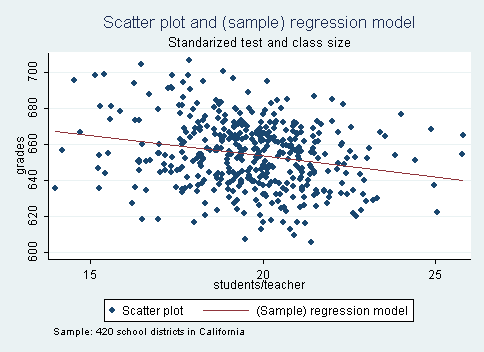
\includegraphics[width=0.75\textwidth]{figures/ols_student_teacher_scores.png}
		\end{figure}
	\end{frame}
	% --------------------------------------------------- Slide --
	\begin{frame} [fragile=singleslide]
		\frametitle{Estimaci\'on MCO: Tama\~no de clase y rendimiento acad\'emico}
		Salida de Stata
		\tiny
			\begin{verbatim}
reg testscr str, robust

Linear regression                                      Number of obs =     420
                                                       F(  1,   418) =   19.26
                                                       Prob > F      =  0.0000
                                                       R-squared     =  0.0512
                                                       Root MSE      =  18.581

------------------------------------------------------------------------------
             |               Robust
     testscr |      Coef.   Std. Err.      t    P>|t|     [95% Conf. Interval]
-------------+----------------------------------------------------------------
     str     |  -2.279808   .5194892    -4.39   0.000    -3.300945   -1.258671
     _cons   |    698.933   10.36436    67.44   0.000     678.5602    719.3057
------------------------------------------------------------------------------
			\end{verbatim}	
		\normalsize
	\end{frame}
	
	% --------------------------------------------------- Slide --
	\begin{frame} [fragile=singleslide]
		\frametitle{Estimaci\'on MCO: Tama\~no de clase y rendimiento acad\'emico}
		Salida de Stata
		\tiny
			\begin{verbatim}
.     reg testscr str  el_pct, robust

Linear regression                                      Number of obs =     420
                                                       F(  2,   417) =  223.82
                                                       Prob > F      =  0.0000
                                                       R-squared     =  0.4264
                                                       Root MSE      =  14.464

------------------------------------------------------------------------------
             |               Robust
     testscr |      Coef.   Std. Err.      t    P>|t|     [95% Conf. Interval]
-------------+----------------------------------------------------------------
         str |  -1.101296   .4328472    -2.54   0.011     -1.95213   -.2504616
      el_pct |  -.6497768   .0310318   -20.94   0.000     -.710775   -.5887786
       _cons |   686.0322   8.728224    78.60   0.000     668.8754     703.189
------------------------------------------------------------------------------
			\end{verbatim}
		\normalsize
		\begin{itemize}
			\item En esta unidad discutimos estimaci\'on puntual, se (robustos!) y $R^2$.
			\item En la siguiente unidad contraste de hip\'otesis (t, F) e intervalos de confianza. 
		\end{itemize}
	\end{frame}
	
%	% --------------------------------------------------- Slide --
%		
%	\section{Causalidad}
%	\begin{frame}
%		\frametitle{Causalidad}
%		\begin{itemize}
%			\item Medir un efecto causal implica realizar un ejercicio contrafactual.
%			\item $d_i$ es una variable binaria que es igual a 1 para tratados 
%			%(alumnos en una clase de menos de 20 estudiantes) 
%			y 0 para no tratados (o grupo de control). 
%			%(alumnos en una clase de m\'as de 20 estudiantes)
%			\item $y_{1i}$ es el resultado en caso que el individuo \alert{fuese} tratado independientemente que sea tratado o no. 
%			%El resultado escolar si el alumno estuviese en una clase de menos de 20 estudiantes independientemente de la clase en que est\'e.
%			\item $y_{0i}$ es el resultado en caso que el individuo \alert{no fuese} tratado independientemente que sea tratado o no.
%			\begin{align*}
%				\text{resultado potencial}= \left\{
%				\begin{array}{l l}
%					y_{1i} & \text{si fuese tratado}\\
%					y_{0i} & \text{si no fuese tratado}
%				\end{array}
%				\right.
%			\end{align*}
%			\item La diferencia es $y_{1i}-y_{0i}$ es el efecto causal individual.
%			\item El resultado observado es $y_i=y_{0i}+(y_{1i}-y_{0i})d_i$
%		\end{itemize}
%	\end{frame}
%	
%	% --------------------------------------------------- Slide --
%	\begin{frame}
%		\frametitle{Causalidad}
%		\small
%		\begin{itemize} 
%			\item Queremos medir el efecto causal medio $\E(y_{1i}-y_{0i})$, \'o el efecto causal medio en tratados $\E(y_{1i}-y_{0i}|d_i=1)$.
%			\item La diferencia de medias observada mide:
%			\begin{align*}
%				\E(y_i&|d_i=1)-\E(y_i|d_i=0)=\\
%				&= \E(y_{1i}|d_i=1)-\E(y_{0i}|d_i=0)\\
%				&= \E(y_{1i}|d_i=1)-\E(y_{0i}|d_i=1)&+&\E(y_{0i}|d_i=1)-\E(y_{0i}|d_i=0)\\
%				&=\underbrace{\E(y_{1i}-y_{0i}|d_i=1)}_\text{\alert{Efecto medio del tratamiento en tratados}} &+& \underbrace{\E(y_{0i}|d_i=1)-\E(y_{0i}|d_i=0)}_\text{\alert{Sesgo de selecci\'on}}
%			\end{align*}
%			\item Si hay \alert{asignaci\'on aleatoria del tratamiento condicional en observables}, entonces $\{y_{1i},y_{0i}\}\independent{d_i}|x_i$ y el sesgo desaparece:
%			\begin{align*}
%				\E(y_i&|d_i=1,x_i)-\E(y_i|d_i=0,x_i)=\E(y_{1i}-y_{0i}|d_i=1,x_i).
%			\end{align*}
%		\end{itemize}
%	\end{frame}

%	% --------------------------------------------------- Slide --
%	\begin{frame}
%		\frametitle{Causalidad}
%		\begin{itemize}
%			\item Introducimos el modelo de regresi\'on.
%			\item Supongamos que los efectos del tratamiento son constantes (iguales para cualquier individuo)
%			\begin{align*}
%				y_{0i}&=\E(y_{0i})+\eta_i=\alpha+\eta_i, \text{ donde } \E(\eta_i)=0\\
%				y_{1i}-y_{0i}&=\rho.
%			\end{align*}
%			\item Podemos escribir
%			\begin{align*}
%				y_{i}&=y_{0i}+(y_{1i}-y_{0i})d_i=\alpha+\rho \, d_i+\eta_i
%			\end{align*}
%			\item Tenemos
%			\begin{align*}
%				\E(\eta_i|d_i=0) = \E(y_{0i}|d_i=0)-\E(y_{0i}) \\
%				\E(\eta_i|d_i=1) = \E(y_{0i}|d_i=1)-\E(y_{0i})
%			\end{align*}
%			\item Si hay sesgo de selecci\'on $\Cov(d_i,\eta_i)\neq 0$
%		\end{itemize}
%	\end{frame}
	
	%% --------------------------------------------------- Slide --
	%\begin{frame}
	%    \frametitle{Causalidad}
	%    \begin{itemize} [<+->]
	%    \item Supuesto de independencia condicional: condicional en caracter\'isticas observadas el sesgo desaparece. $\{y_{1i},y_{0i}\}\independent{d_i}|x_i$
	%    \item Modelo de regresi\'on: Suponemos efecto causal constante
	%    \begin{align*}
	%    y_{0i}&=\alpha+v_i,\\
	%    y_{1i}-y_{0i}&=\rho.
	%    \end{align*}
	%    \item Entonces $y_i=\alpha+\rho d_i+v_i$
	%    \item Suponga que $\E(v_i|x_i)=\gamma'x_i$. Esto implica que $\E(y_{0i}|x_i,d_i)=\alpha+x_i'\gamma$.
	%    \item Entonces $\E(y_{i}|x_i,d_i)=\alpha+\rho \,d_i+x_i'\gamma$.
	%    \item Por lo tanto, tenemos $y_{i}=\alpha+\rho \,d_i+x_i'\gamma+u_i$,
	%    con $u_i$ incorrelado con $d_i$ y $x_i$.
	%    \end{itemize}
	%\end{frame}
	% --------------------------------------------------- Slide --
	\section{Modelo de regresi\'on lineal: Supuestos}
	\begin{frame}
		\frametitle{Modelo de regresi\'on lineal}
 			\begin{align*}
				y_i&=\beta_0 + \beta_1 x_{1i} + ...+\beta_K  x_{Ki}+u_i \\
				&= x_i'\beta+u_i,
			\end{align*}
			donde $y_i$ es una variable aleatoria (escalar), $x_i$ es un vector aleatorio de $K \times 1$ (para no tener que trabajar con $K+1$) y $u_i$ es una variable aleatoria (escalar).
	\end{frame}
	\begin{frame}
		\frametitle{Modelo de regresi\'on lineal}
 			\begin{align*}
				y_i = x_i'\beta+u_i
			\end{align*}
		\begin{itemize}
 			\item \alert{Supuestos}:
			\begin{enumerate}
				\bigskip
				\item [OLS1] Muestra aleatoria de tama\~no $N$ $\implies \{y_i,x_i\}_{i=1}^N$ i.i.d.
				\bigskip
				\item [OLS2]  No correlaci\'on entre las variables explicativas y el inobservado: $\E(x_iu_i)=0$.
				\bigskip
				\item [OLS3]  No colinealidad perfecta entre las variables explicativas: $\E(x_ix_i')$ es invertible o $\text{rango}(\E(x_ix_i'))=K$.
				\bigskip
				\item [OLS4]  Condiciones de regularidad (``No fat tails''): $\E(||x_i||^4)<\infty$ y $\E(y_i^4)<\infty$.
			\end{enumerate}
			% Muestra aleatoria: Razonable para datos de seccion cruzada (transversales) y datos de panel (longitudinales). No es razonable para series temporales.
			% No correlaci\'on: No asumimos x fijas, x independiente de u, u independiente en media de x.
			% No multicolinealidad perfecta: No hay una relaci\'on lineal entre las variables incluidas en la regresi\'on. No cumple cuando usamos una dummy para cada categoria de una variable discreta y la constante, una dummy y la dummy al cuadrado, usamos logx y log (x^2)(=2log x). Si no hay multicolinealidad perfecta, se puede utilizar MCO pero es dificil obtener una estiamci\'on precisa de los betas.
			% No fat tails: Utilizamos estas condiciones cuando necesitamos un estiamdor consistente de la matriz de varianza y covarianza. Son supuestos t\'ecnicos o de regularidad, y los incluimos para hacer la exposicion rigurosa.
			% No asumimos 1. Normalidad de u, 2. Homoscedasticidad.
		\end{itemize}
	\end{frame}

%	\begin{frame}
%	\end{frame}
%
%	\begin{frame}
%	\end{frame}

	% --------------------------------------------------- Slide --

	\section{Identificaci\'on}
	\begin{frame}
		\frametitle{Identificaci\'on}
		\begin{itemize}
			\item  Escribir los par\'ametros como una funci\'on de momentos poblacionales: ?`Qu\'e momentos poblacionales permiten \alert{identificar} los par\'ametros de inter\'es?
		\end{itemize}
	\end{frame}

%	\begin{frame}
%		\frametitle{Identificaci\'on}
%	\end{frame}

	\begin{frame}
		\frametitle{Identificaci\'on}
		\begin{itemize}
			\item  Escribir los par\'ametros como una funci\'on de momentos poblacionales: ?`Qu\'e momentos poblacionales permiten \alert{identificar} los par\'ametros de inter\'es?
			\begin{align*}
				&\E(x_iu_i)=0 \quad \text{usando OLS2},\\
				&\iff \E[x_i(y_i-x_i'\beta)] =0,\\
				&\iff \E(x_iy_i)-\E(x_ix_i')\beta=0,\\
				&\iff \beta =\E(x_ix_i')^{-1}\E(x_iy_i)\quad \text{usando OLS3}.
			\end{align*}
			\item OLS2 y OLS3 son los supuestos que identifican $\beta$.
		\end{itemize}
	\end{frame}
	% Alguna intuicion sobre la idea de identificaci\'on es necesaria
	% --------------------------------------------------- Slide --
	\section{Estimaci\'on por M\'inimos Cuadrados Ordinarios (OLS)}
	\begin{frame}
		\frametitle{M\'inimos Cuadrados Ordinarios (OLS)}
		\begin{itemize}
			\item  \alert{Principio de analog\'ia}: reemplazar momentos poblacionales por momentos muestrales.
			\item [] <2->Estamos interesados en:
			\begin{align*}
				\beta =\E(x_ix_i')^{-1}\E(x_iy_i).
			\end{align*}
			Usando el principio de analog\'ia, lo estimamos con
			\begin{align*}
				\hat \beta =\left(\frac{1}{N}\sum_{i=1}^{N} x_ix_i'\right)^{-1} \frac{1}{N} \sum_{i=1}^{N}x_iy_i.
			\end{align*}
		\end{itemize}
	\end{frame}
	% El principio de analogia nos da la intuicion que lo que se verifica en la poblacion ahora se verifica en la muestra si reemplazamos momentos poblacionales por momentos muestrales: Cov(u,x)=0.
	% Interpretacion como minimiza desvios al cuadrado
	% --------------------------------------------------- Slide --
	\begin{frame}
		\frametitle{M\'inimos Cuadrados Ordinarios (OLS)}
		\begin{itemize}
			\item  \alert{M\'etodo de momentos}: 			
			\item [] <2->El modelo poblacional cumple 
			\begin{align*}
				\E[x_i(y_i-x_i'\beta)]=0.
			\end{align*}
			El estimador satisface una condici\'on similar en la muestra 
			\begin{align*}
				\frac{1}{N}\sum_{i=1}^{N} x_i(y_i-x_i'\hat \beta)=0.
			\end{align*}
			\item <2-> Note que
			\begin{align*}
			  \Cov(x_i,u_i) &= \Cov(x_i,y_i-x_i' \beta) = 0, \\
			  \alert{\widehat{\Cov}}(x_i,\alert{\hat u_i}) &= \alert{\widehat{\Cov}}(x_i,y_i-x_i'\alert{\hat \beta})= 0.
			\end{align*}
		\end{itemize}
	\end{frame}
	% El principio de analogia nos da la intuicion que lo que se verifica en la poblacion ahora se verifica en la muestra si reemplazamos momentos poblacionales por momentos muestrales: Cov(u,x)=0.
	% Interpretacion como minimiza desvios al cuadrado
	% --------------------------------------------------- Slide --
	\begin{frame}
		\frametitle{M\'inimos Cuadrados Ordinarios (OLS)}
		\begin{align*}
			\hat \beta =\left(\frac{1}{N}\sum_{i=1}^{N} x_ix_i'\right)^{-1} \frac{1}{N} \sum_{i=1}^{N}x_iy_i.
		\end{align*}
		\begin{itemize}
			\item En forma matricial
			\begin{align*}
				\hat \beta =(X'X)^{-1}(X'y),
			\end{align*}
			donde $X$ es una matriz de $N \times K$ e $y$ es un vector de $N \times 1$ dados por
			\begin{align*}
				X =\left(
				\begin{array} {c}
					x_1'   \\
					\vdots \\
					x_N'
				\end{array}
				\right)
				\quad \text{e} \quad
				y =\left(
				\begin{array} {c}
					y_1   \\
					\vdots \\
					y_N
				\end{array}
				\right)
			\end{align*}
		\end{itemize}
	\end{frame}
	% Bajo el supuesto de muestreo aleatorio, la forma matricial solamente es \'util para computar OLS, y para propiedades en muestras peque\~nas (irrelevante en la pr\'actica).
	% --------------------------------------------------- Slide --
	\begin{frame}
		\frametitle{Modelo de regresi\'on simple}
		\begin{itemize}
			\item []
			\begin{align*}
				y_i = \beta_0 + \beta_1 x_{1i}+u_i,
			\end{align*}
			donde
			\begin{align*}
				\beta_1 &= \frac{\Cov(x_{1i}, y_i)}{\Var(x_{1i})},\\
				\beta_0 &= \E(y_i)-\beta_1\E(x_{1i}).
			\end{align*}
		\end{itemize}
	\end{frame}
%	
%	\begin{frame}
%	\end{frame}
%	
%	\begin{frame}
%	\end{frame}
	
	\begin{frame}
		\frametitle{Modelo de regresi\'on simple}
		\begin{itemize}
			\item []
			\begin{align*}
				y_i = \beta_0 + \beta_1 x_{1i}+u_i,
			\end{align*}
			donde
			\begin{align*}
				\beta_1 &= \frac{\Cov(x_{1i}, y_i)}{\Var(x_{1i})},\\
				\beta_0 &= \E(y_i)-\beta_1\E(x_{1i}).
			\end{align*}
			El estimador OLS es,
				\begin{align*}
					\hat \beta_1 &=\frac{\frac{1}{N}\sum_{i=1}^{N} x_{1i}(y_{i}-\bar y)}{\frac{1}{N}\sum_{i=1}^{N} x_{1i}(x_{1i}-\bar x_1)}=\frac{\frac{1}{N}\sum_{i=1}^{N} y_{i}(x_{1i}-\bar x_1)}{\frac{1}{N}\sum_{i=1}^{N} x_{1i}(x_{1i}-\bar x_1)} =\frac{\widehat{\Cov}(x_{1i},y_i)}{\widehat{\Var}(x_{1i})}, \\
					\hat \beta_0 &=\bar y - \hat \beta_1 \bar x_1.
				\end{align*}
		\end{itemize}
	\end{frame}
	% Demostraci\'on: Utilizar el principio de analog\'ia o trabajar con la f\'ormula general.
	% --------------------------------------------------- Slide --
	\begin{frame}
		\frametitle{Regresi\'on particionada}
		\begin{itemize}
			\item <1->[] Dado el modelo de regresi\'on m\'ultiple
			\begin{align*}
				y_i = \beta_0+\beta_1x_{1i}+...+\beta_k x_{ki} +...+\beta_K x_{Ki}+ u_i.
			\end{align*}
			Podemos estimar $\beta_1$ a partir de:
			\begin{align*}
				\hat \beta_{1} = \frac{\widehat{\Cov}(\tilde x_{1i},y_i)}{\widehat{\Var}(\tilde x_{1i})},
			\end{align*}
			donde
			\begin{align*}
				x_{1i} = \sum_{j\neq 1} \hat \gamma_j \, x_{ji}+\tilde x_{1i} =\hat x_{1i}+\tilde x_{1i}.
			\end{align*}
		\end{itemize}
	\end{frame}
	% --------------------------------------------------- Slide --
	\begin{frame}
		\frametitle{Regresi\'on particionada}
		\begin{itemize}
			\item <1-> Demostraci\'on: 
			\begin{align*}
				\hat \beta_{1} & = \frac{\widehat{\Cov}(\tilde x_{1i},y_i)}{\widehat{\Var}(\tilde x_{1i})},\\
				& = \frac{\widehat{\Cov}(\tilde x_{1i},\hat\beta_0+\hat\beta_1x_{1i}+...+\hat\beta_K x_{Ki}+ \hat u_i)}{\widehat{\Var}(\tilde x_{1i})}.
			\end{align*}
			\begin{enumerate}
				\item[(1)] $\widehat{\Cov}(\tilde x_{1i},x_{ji})=0$ para todo $j\neq 1$, por construcci\'on,
				\item[(2)] $\widehat{\Cov}(\tilde x_{1i},\hat u_i)=0$ porque $\hat u_i$ no est\'a correlado con $x_i$'s y $\tilde x_{1i}$ es una funci\'on lineal de $x_i$'s.
			\end{enumerate}
			Entonces,
			\small
			\begin{align*}
				\frac{\widehat{\Cov}(\tilde x_{1i},y_{i})}{\widehat{\Var}(\tilde x_{1i})} & = \hat \beta_1\frac{\widehat{\Cov}(\tilde x_{1i},x_{1i})}{\widehat{\Var}(\tilde x_{1i})}
				= \hat \beta_1\frac{\widehat{\Cov}(\tilde x_{1i},\hat x_{1i}+\tilde x_{1i})}{\widehat{\Var}(\tilde x_{1i})}
				= \hat \beta_1\frac{\widehat{\Cov}(\tilde x_{1i},\tilde x_{1i})}{\widehat{\Var}(\tilde x_{1i})}=\hat \beta_1.
			\end{align*}
		\end{itemize}
	\end{frame}
	% --------------------------------------------------- Slide --
	\begin{frame}
		\frametitle{Predicci\'on}
		\begin{itemize}
			\item  Los coeficientes $\beta$ de la regresi\'on poblacional se pueden definir como la soluci\'on del problema de m\'inimos cuadrados en la poblaci\'on:
			\begin{align*}
				\beta = \arg \min_b \E[(y_i-x_i'b)^2].
			\end{align*}
			\item Los estimadores por OLS $\hat \beta $ de $\beta$ se pueden definir como la soluci\'on del problema de m\'inimos cuadrados en la muestra:
			\begin{align*}
				\hat \beta = \arg \min_b \frac{1}{N}\sum_{i=1}^{N}(y_i-x_i'b)^2.  
			\end{align*}
			\bigskip
			Utilizando las condiciones de primer orden
			\begin{align*}
				\frac{1}{N}\sum_{i=1}^{N} x_i(y_i-x_i'\hat \beta)=0 \implies \hat \beta= \left(\frac{1}{N}\sum_{i=1}^{N} x_ix_i'\right)^{-1}\frac{1}{N}\sum_{i=1}^{N}x_i y_i.
			\end{align*}
		\end{itemize}
	\end{frame}
%
%	\begin{frame}
%	\end{frame}
		
	
	% --------------------------------------------------- Slide --
	\section{Propiedades}
	
%	\begin{frame}
%		\frametitle{Propiedades: Consistencia $\plim \hat \beta=\beta$}
%	\end{frame}
%	
%	\begin{frame}
%		\frametitle{Propiedades: Consistencia $\plim \hat \beta=\beta$}
%	\end{frame}
%
%	\begin{frame}
%		\frametitle{Propiedades: Consistencia $\plim \hat \beta=\beta$}
%	\end{frame}

	\begin{frame}
		\frametitle{Propiedades: Consistencia $\plim \hat \beta=\beta$}
		\begin{itemize}
		    \small
			\item \alert{Paso intermedio}
			\begin{align*}
				\hat\beta & = \left( \frac{1}{N}\sum_{i=1}^{N}x_ix_i'\right)^{-1}\left( \frac{1}{N}\sum_{i=1}^{N}x_iy_i\right) = \beta + \left( \frac{1}{N}\sum_{i=1}^{N}x_ix_i'\right)^{-1}\left( \frac{1}{N}\sum_{i=1}^{N}x_iu_i\right)
			\end{align*}
			\item \alert{Demostraci\'on}
			\begin{align*}
				\plim \hat \beta & = \plim \beta +  \left( \plim \frac{1}{N}\sum_{i=1}^{N}x_ix_i'\right)^{-1}\plim\left( \frac{1}{N}\sum_{i=1}^{N}x_iu_i\right)= \beta,
			\end{align*}
			usando LGN y TFC en
			\begin{align*}
				\plim\left(  \frac{1}{N}\sum_{i=1}^{N}x_ix_i'\right)& = \E(x_ix_i'), \\
				\plim \frac{1}{N}\sum_{i=1}^{N}x_iu_i & = \E(x_iu_i)=0,
			\end{align*}
		\end{itemize}
	\end{frame}
	
	% --------------------------------------------------- Slide --
	\begin{frame}
		\frametitle{Repaso: Matriz de varianzas-covarianzas}
		\begin{itemize}
			\item Dada una variable aleatoria $y$ su varianza es $\Var(y)=\E[(y-\E y)^2]=\E(y^2)-(\E y)^2$.
			\item Dada un vector de variables aleatorias $\mathbf{y}$ su matrix de varianzas-covarianzas es 
			\begin{align*}
			  \Var(\mathbf{y})=\E[(\mathbf{y}-\E \mathbf{y})(\mathbf{y}-\E \mathbf{y})']=\E(\mathbf{y}\mathbf{y}')-(\E \mathbf{y})(\E \mathbf{y})'.
			\end{align*}
			\item Ejemplo: $\mathbf{y} = (y_1\quad  y_2)'$.	
		\end{itemize}
	\end{frame}
	% --------------------------------------------------- Slide --
%	\begin{frame}
%		\frametitle{Propiedades: Distribuci\'on asint\'otica normal}
%	\end{frame}
%	
%	\begin{frame}
%		\frametitle{Propiedades: Distribuci\'on asint\'otica normal}
%	\end{frame}
%
%	\begin{frame}
%		\frametitle{Propiedades: Distribuci\'on asint\'otica normal}
%	\end{frame}
	
	\begin{frame}
		\frametitle{Propiedades: Distribuci\'on asint\'otica normal}
		\begin{itemize}
			\item \alert{Demostraci\'on}
			\begin{align*}
				\sqrt{N} (\hat \beta - \beta)&= \left( \frac{1}{N}\sum_{i=1}^{N}x_ix_i'\right)^{-1} \sqrt{N}\frac{1}{N}\sum_{i=1}^{N}x_iu_i.
			\end{align*}
			Usando LGN+TFC y TCL en,
			\begin{align*}
				\plim\left(  \frac{1}{N}\sum_{i=1}^{N}x_ix_i'\right)^{-1}& = \E(x_ix_i')^{-1},\\
				\sqrt{N}\frac{1}{N}\sum_{i=1}^{N}x_iu_i &\dto \N (0,\E(u_i^2 x_i x_i')).
			\end{align*}
			Usando el teorema de Slutsky
			\begin{align*}
				\sqrt{N} (\hat \beta - \beta) &\dto \N (0,\E(x_ix_i')^{-1}\E(u_i^2 x_i x_i')\E(x_ix_i')^{-1}).
			\end{align*}
		\end{itemize}
	\end{frame}
	% --------------------------------------------------- Slide --
	\begin{frame}
		\frametitle{Propiedades: Distribuci\'on asint\'otica normal}
		\begin{align*}
			\sqrt{N} (\hat \beta - \beta) &\dto \N (0,\E(x_ix_i')^{-1}\E(u_i^2 x_i x_i')\E(x_ix_i')^{-1}),
		\end{align*}
		donde $\E(u_i^2 x_i x_i')<\infty$ bajo el supuesto $\E(||x_i||^4)<\infty$ y $\E(y_i^4)<\infty$.
		\begin{itemize}
			\item Decimos
			\begin{align*}
				&\hat \beta \adistr \N(\beta,\Avar(\hat\beta)),\text{ donde}\\
				&\Avar(\hat\beta)=\frac{1}{N}\E(x_ix_i')^{-1}\E(u_i^2 x_i x_i')\E(x_ix_i')^{-1}.
			\end{align*}
		\end{itemize}
	\end{frame}
	
	\begin{frame}
		\frametitle{Ejemplo: Modelo de regresi\'on simple}
		\small
		\begin{itemize}
			\item[]
			\begin{align*}
				y_i = \beta_0 + \beta_1 x_{1i}+u_i,
			\end{align*}
			donde $\E(u_i)=\E(x_{1i}u_i)=0$
			\item[] El estimador OLS es,
			\begin{align*}
				\hat \beta_1 & =\frac{\frac{1}{N}\sum_{i=1}^{N} y_{i}(x_{1i}-\bar x_1)}{\frac{1}{N}\sum_{i=1}^{N} x_{1i}(x_{1i}-\bar x_1)}=\frac{\widehat{\Cov}(x_{1i},y_i)}{\widehat{\Var}(x_{1i})}.
				\end{align*}
		\end{itemize}
	\end{frame}
	
%	\begin{frame}
%	\end{frame}
%	
%	\begin{frame}
%	\end{frame}
%	
%	\begin{frame}
%	\end{frame}
	
	\begin{frame}
		\frametitle{Ejemplo: Modelo de regresi\'on simple}
		\vspace{-.5cm}
		\small
		\begin{itemize}
			\item[]
			\begin{align*}
				y_i = \beta_0 + \beta_1 x_{1i}+u_i,
			\end{align*}
			donde $\E(u_i)=\E(x_{1i}u_i)=0$
			\item[] El estimador OLS es,
			\begin{align*}
				\hat \beta_1 & =\frac{\frac{1}{N}\sum_{i=1}^{N} y_{i}(x_{1i}-\bar x_1)}{\frac{1}{N}\sum_{i=1}^{N} x_{1i}(x_{1i}-\bar x_1)}=\frac{\widehat{\Cov}(x_{1i},y_i)}{\widehat{\Var}(x_{1i})}.
				\end{align*}
			\item La distribuci\'on asint\'otica es
			\begin{align*}
				\sqrt{N} (\hat \beta_1 - \beta_1) &\dto \N (0,\frac{\E[u^2(x_1 -\E (x_1))^2]}{\Var(x_1)^2}),
			\end{align*}				
			\item Decimos
			\begin{align*}
				&\hat \beta_1 \adistr \N(\beta_1,\Avar(\hat\beta_1)),\text{ donde}\\
				&\Avar(\hat\beta_1)=\frac{1}{N}\frac{\E[u^2(x_1 -\E (x_1))^2]}{\Var(x_1)^2}.
			\end{align*}
		\end{itemize}
	\end{frame}

%	\begin{frame}
%		\frametitle{Repaso}
%	\end{frame}
%
%	\begin{frame}
%		\frametitle{Repaso}
%	\end{frame}

	% --------------------------------------------------- Slide --
	\section{Homoscedasticidad}

%	\begin{frame}
%		\frametitle{Homoscedasticidad: $\E(u_i^2|x_i) = \E(u_i^2) = \sigma^2$}
%	\end{frame}
%	
%	\begin{frame}
%		\frametitle{Homoscedasticidad: $\E(u_i^2|x_i) = \E(u_i^2) = \sigma^2$}
%	\end{frame}

	\begin{frame}
		\frametitle{Homoscedasticidad: $\E(u_i^2|x_i) = \E(u_i^2) = \sigma^2$}
		\begin{itemize}
			\item Entonces
			\begin{align*}
				\E(u_i^2 x_i x_i') = \E[\E(u_i^2|x_i) x_i x_i']=\sigma^2\E(x_i x_i'),
			\end{align*}
			Por lo tanto
			\begin{align*}
				\Avar(\hat \beta)&=\frac{1}{N}\E(x_ix_i')^{-1}\E(u_i^2 x_i x_i')\E(x_ix_i')^{-1},\\
				&=\frac{1}{N}\E(x_ix_i')^{-1}\sigma^2\E(x_i x_i')\E(x_ix_i')^{-1},\\
				&=\frac{\sigma^2}{N}\E(x_ix_i')^{-1}.
			\end{align*}
		\end{itemize}
	\end{frame}
	% --------------------------------------------------- Slide --
	\begin{frame}
		\frametitle{Homoscedasticidad}
		\begin{itemize}
			\item En el modelo de regresi\'on simple $y_i=\beta_0+\beta_1x_{1i}+u_i$:
			\begin{align*}
				\Avar(\hat \beta_1)&=\frac{\E(u_i^2)}{N}\frac{1}{\Var(x_{1i})}.
			\end{align*}
			\item [] Interpretaci\'on
		\end{itemize}
	\end{frame}

%	\begin{frame}
%		\frametitle{Homoscedasticidad}
%	\end{frame}
%	
%
%	\begin{frame}
%		\frametitle{Homoscedasticidad}
%	\end{frame}
	
	\begin{frame}
		\frametitle{Homoscedasticidad}
		\begin{itemize}
			\item En el modelo de regresi\'on m\'ultiple
			\begin{align*}
				y_i = \beta_0+\beta_1x_{1i}+...+\beta_k x_{ki} +...+\beta_K x_{Ki}+ v_i.
			\end{align*}
			Usando la regresi\'on particionada,
			\begin{align*}
				\Avar(\hat \beta_1)&=\frac{\E(v_i^2)}{N}\frac{1}{\Var(\tilde x_{1i})}.
			\end{align*}
		\end{itemize}
	\end{frame}
		
%	\begin{frame}
%		\frametitle{Homoscedasticidad}
%	\end{frame}
%
%	\begin{frame}
%		\frametitle{Homoscedasticidad}
%	\end{frame}
%	
	\begin{frame}
		\frametitle{Homoscedasticidad}
		\begin{itemize}
			\item En el modelo de regresi\'on simple $y_i=\beta_0+\beta_1x_{1i}+u_i$:
			\begin{align*}
				\Avar(\hat \beta_1)&=\frac{\E(u_i^2)}{N}\frac{1}{\Var(x_{1i})}.
			\end{align*}
			\item En el modelo de regresi\'on m\'ultiple
			\begin{align*}
				y_i = \beta_0+\beta_1x_{1i}+...+\beta_k x_{ki} +...+\beta_K x_{Ki}+ v_i.
			\end{align*}
			\begin{align*}
				\Avar(\hat \beta_1)&=\frac{\E(v_i^2)}{N}\frac{1}{\Var(\tilde x_{1i})}.
			\end{align*}					
			\item \alert{Comparar}
		\end{itemize}
	\end{frame}
	
		% --------------------------------------------------- Slide --
	\begin{frame}
		\frametitle{Homoscedasticidad}
		Si la esperanza condicional no es lineal, entonces el modelo de regresi\'on es heterosced\'astico. (Incluso si  $\Var(y_i|x_i)$ es constante.)
	\end{frame}

%	\begin{frame}
%		\frametitle{Homoscedasticidad}
%	\end{frame}
%
%	\begin{frame}
%		\frametitle{Homoscedasticidad}
%	\end{frame}

	\begin{frame}
		\frametitle{Homoscedasticidad}
		Si la esperanza condicional no es lineal, entonces el modelo de regresi\'on es heterosced\'astico. (Incluso si  $\Var(y_i|x_i)$ es constante.)
		\begin{itemize}
		    \small
			\item \alert{Demostraci\'on}:
			\begin{align*}
				\E(u_i^2|x_i) & =\E((y_i-x_i'\beta)^2|x_i),\\
				& = \E\{[(y_i-\E(y_i|x_i))+(\E(y_i|x_i)-x_i'\beta)]^2|x_i\},\\
				& = \E[(y_i-\E(y_i|x_i))^2|x_i]+\E[(\E(y_i|x_i)-x_i'\beta)^2|x_i],\\
				& = \Var(y_i|x_i)+\E[(\E(y_i|x_i)-x_i'\beta)^2|x_i].
			\end{align*}
			Inclusive si $\Var(y_i|x_i)$ es constante, $\E(u_i^2|x_i)$  depende de $x_i$ seg\'un el modelo de regresi\'on sea una mejor o peor aproximaci\'on a la esperanza condicional para distintos valores de $x_i$.
			\item Concluimos que el supuesto de homoscedasticidad es poco probable que se cumpla en la pr\'actica.
		\end{itemize}
	\end{frame}
	
    \begin{frame}
        \frametitle{Ejemplo: Educaci\'on y salarios en US}
        \vspace{-.5cm}
        \begin{figure}
            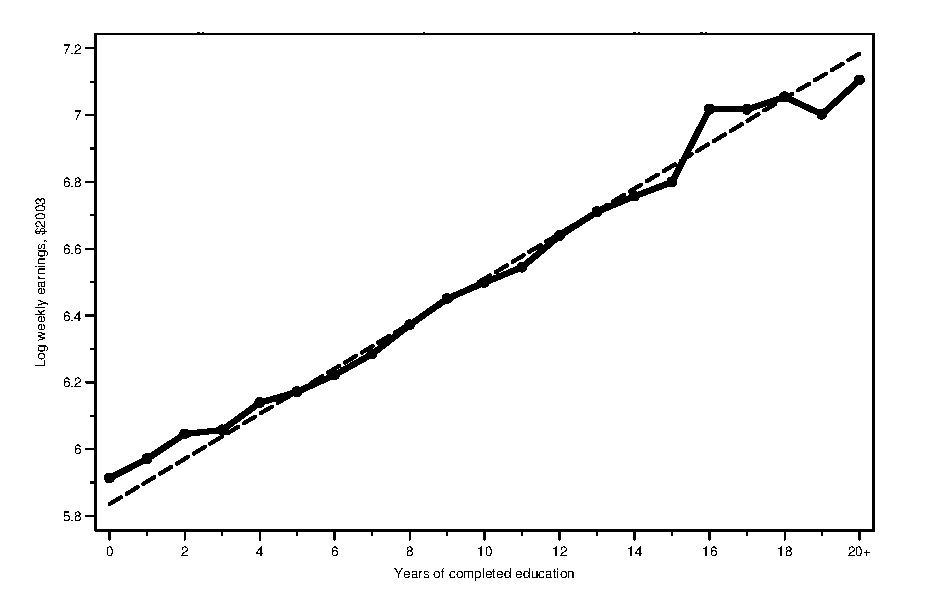
\includegraphics[width=0.65\textwidth]{figures/AP_figure_educacion_salarios_regresion.pdf}
            \caption{Regresi\'on y esperanza condicional del log salarios semanales en el nivel educativo. La muestra incluye hombres blancos entre 40 y 49 a\~nos de la muestra del 5\% del Censo 1980 (IPUMS).}
        \end{figure}
    \end{frame}
	
	% --------------------------------------------------- Slide --\begin{frame}
	\begin{frame}
		\frametitle{Propiedades en muestras peque\~nas: Insesgadez}
		Si suponemos $\E(u_i|x_i)=0$ entonces $\E(\hat \beta)=\beta$ donde $X=(x_1,...,x_N)$.
	\end{frame}
	
%	\begin{frame}
%	\end{frame}
%	
%	\begin{frame}
%	\end{frame}

	\begin{frame}
		\frametitle{Propiedades en muestras peque\~nas: Insesgadez}
		Si suponemos $\E(u_i|x_i)=0$ entonces $\E(\hat \beta)=\beta$ donde $X=(x_1,...,x_N)$.
		\begin{itemize}
			\item Demostraci\'on:
			\begin{align*}
				\E(\hat \beta |X) &= \beta +  \left( \frac{1}{N}\sum_{i=1}^{N}x_ix_i'\right)^{-1} \frac{1}{N}\sum_{i=1}^{N}x_i\E(u_i|x_i)= \beta,
			\end{align*}
			usando $\E(u_i|X)=\E(u_i|x_i)$ por el supuesto iid y $\E(u_i|x_i)=0$.\\
			Luego por la LEI
			\begin{align*}
				\E(\hat \beta) & = \E[\E(\hat \beta |X)] =\E(\beta)=\beta.
			\end{align*}
		\end{itemize}
	\end{frame}
	
	% --------------------------------------------------- Slide --
	\begin{frame}
		\frametitle{Teorema de Gauss-Markov}
		Si $\E(u_i|x_i)=0$ y $\E(u_i^2|x_i)=\sigma^2$ (homoscedasticidad), entonces $\hat \beta$ es el estimador de menor varianza (condicional en $X$) entre los estimadores insesgados y lineales en $y$.
		\begin{itemize}
			\item <2-> Demostraci\'on (sketch): Calculamos la varianza condicional
			\footnotesize
			\begin{align*}
				\Var&(\hat \beta|X) = \E[(\hat \beta-\beta)(\hat \beta-\beta)'|X],\\
				&= \left( \frac{1}{N}\sum_{i=1}^{N}x_ix_i'\right)^{-1}\E\left[\left( \frac{1}{N}\sum_{i=1}^{N}x_iu_i\right)\left( \frac{1}{N}\sum_{i=1}^{N}x_i'u_i\right)|X\right]\left( \frac{1}{N}\sum_{i=1}^{N}x_ix_i'\right)^{-1},\\
				&= \left( \frac{1}{N}\sum_{i=1}^{N}x_ix_i'\right)^{-1}\E\left[\left( \frac{1}{N^2}\sum_{i=1}^{N}x_ix_i'u_i^2\right)|X\right]\left( \frac{1}{N}\sum_{i=1}^{N}x_ix_i'\right)^{-1},\\
				&= \left( \frac{1}{N}\sum_{i=1}^{N}x_ix_i'\right)^{-1}\left( \frac{1}{N^2}\sum_{i=1}^{N}x_ix_i'\E(u_i^2|x_i)\right)\left( \frac{1}{N}\sum_{i=1}^{N}x_ix_i'\right)^{-1},\\
				&= \frac{\sigma^2}{N}\left( \frac{1}{N}\sum_{i=1}^{N}x_ix_i'\right)^{-1}.
			\end{align*}
		\end{itemize}
	\end{frame}
	% Este resultado es para cualquier N.
	%La varianza obtiene la cota Cramer-Rao por lo tanto no existe otro estiamdor insesgado de menor varianza.
	% Usamos que dada que la muestra es iid \E(u_iu_j|X)=\E(u_i|X)\E(u_j|X)=\E(u_i|x_i)\E(u_j|x_j)=0
	
	% --------------------------------------------------- Slide --
	\begin{frame}
		\frametitle{Teorema de Gauss-Markov}
		Si $\hat \beta$ minimiza la varianza condicional $\Var(b|X)$ entonces minimiza la varianza no condicional $\Var(b)$, donde $b$ son estimadores insesgados de $\beta$.
		\begin{itemize}
			\item  <2->  Demostraci\'on: Sabemos que 
			\begin{align*}
				\Var(\hat \beta|X)\leq \Var(b|X)
			\end{align*} 
			donde $b$ es un estimador insesgado de $\beta$. Utilizando la descomposici\'on de varianza
			\begin{align*}
				\Var(b)=\E[\Var(b|X)]+\Var[\E(b|X)].
			\end{align*} 
			Pero hemos demostrado anteriormente que:
			\begin{align*}
				\Var[\E(\hat \beta|X)]&=\Var(\beta)=0.
			\end{align*}
			Entonces $\Var(\hat \beta|X) \leq \Var(b|X) \implies \Var(\hat \beta)\leq \Var(b)$ donde $b$ es un estimador insesgado de $\beta$.
		\end{itemize}
	\end{frame}
		
	% --------------------------------------------------- Slide --
	\section{Estimaci\'on de la matriz de varianzas-covarianzas}
	\begin{frame}
		\frametitle{Estimaci\'on de la matriz de varianzas-covarianzas}
		\begin{itemize}
			\item Supongamos homoscedasticidad $\E(u_i^2|x_i) = \sigma^2$.
			\item [] Estamos interesados en un estimador consistente de 
			\begin{align*}
				\Avar(\sqrt{N} (\hat \beta - \beta))=\sigma^2\E(x_ix_i')^{-1}.
			\end{align*}
			\item <2-> [] Puede ser una buena idea usar:
			\small{
				\begin{align*}
					\widehat{\Avar}(\sqrt{N} (\hat \beta - \beta))&= \left(\frac{1}{N}\sum_{i=1}^{N}\hat u_i^2 \right)\left( \frac{1}{N}\sum_{i=1}^{N}x_ix_i'\right)^{-1}= \hat\sigma^2\left( \frac{1}{N}\sum_{i=1}^{N}x_ix_i'\right)^{-1},
				\end{align*}
			}
			donde $\hat u_i=y_i -x_i'\hat \beta$.
			\item <3->[] \alert{Demostraci\'on}: Anteriormente demostramos que 
			\begin{align*}
				\plim \left( \frac{1}{N}\sum_{i=1}^{N}x_ix_i'\right)^{-1} = \E(x_ix_i')^{-1},
			\end{align*}
			nos queda demostrar que $\plim\hat \sigma^2 = \sigma^2$.
		\end{itemize}
	\end{frame}
	
	% --------------------------------------------------- Slide --
	\begin{frame}
		\frametitle{Homoscedasticidad}
		\begin{itemize}
			\item <1-> Nos queda demostrar que $\plim \hat \sigma^2 = \sigma^2$:
		\end{itemize}
	\end{frame}
	
%	\begin{frame}
%		\frametitle{Homoscedasticidad}
%	\end{frame}
%
%	\begin{frame}
%		\frametitle{Homoscedasticidad}
%	\end{frame}
%
%	\begin{frame}
%		\frametitle{Homoscedasticidad}
%	\end{frame}
	
	% --------------------------------------------------- Slide --
	\begin{frame}
		\frametitle{Homoscedasticidad}
		\begin{itemize}
			\item <1-> Nos queda demostrar que $\plim \hat \sigma^2 = \sigma^2$:
			\small
			\begin{align*}
				\frac{1}{N}&\sum_{i=1}^{N}\hat u_i^2  = \frac{1}{N}\sum_{i=1}^{N}(y_i-x_i'\hat \beta)^2,\\
				& = \frac{1}{N}\sum_{i=1}^{N} [(y_i-x_i'\beta)-(x_i'\hat \beta-x_i'\beta)]^2,\\
				& = \frac{1}{N}\sum_{i=1}^{N} [(y_i-x_i'\beta)^2+(x_i'\hat \beta-x_i'\beta)^2
				-2(x_i'\hat \beta-x_i'\beta)(y_i-x_i'\beta)],\\
				& = \frac{1}{N}\sum_{i=1}^{N} [u_i^2+(\hat \beta-\beta)'x_ix_i'(\hat \beta-\beta)
				-2 (\hat \beta-\beta)'x_i u_i],\\
				& = \frac{1}{N}\sum_{i=1}^{N} u_i^2+(\hat \beta-\beta)'\left(\frac{1}{N}\sum_{i=1}^{N}x_ix_i'\right)(\hat \beta-\beta)
				-2 (\hat \beta-\beta)'\frac{1}{N}\sum_{i=1}^{N}x_i u_i.
			\end{align*}
		\end{itemize}
	\end{frame}
	% --------------------------------------------------- Slide --
	\begin{frame}
		\frametitle{Homoscedasticidad}
		\begin{itemize}
			\item Nos queda demostrar $\plim\frac{1}{N}\sum_{i=1}^{N}\hat u_i^2 = \sigma^2$:
			\footnotesize{
				\begin{align*}
					\frac{1}{N}\sum_{i=1}^{N}\hat u_i^2 & =\frac{1}{N}\sum_{i=1}^{N} u_i^2+(\hat \beta-\beta)'\left(\frac{1}{N}\sum_{i=1}^{N}x_ix_i'\right)(\hat \beta-\beta)
					-2 (\hat \beta-\beta)'\frac{1}{N}\sum_{i=1}^{N}x_i u_i.
				\end{align*}
			}
			\item [] Utilizando LGN y TFC
			\small{
				\begin{align*}
					\plim \frac{1}{N}\sum_{i=1}^{N}u_i^2 & =\E(u_i^2)=\sigma^2,\\
					\plim(\hat \beta-\beta)'\plim \left(\frac{1}{N}\sum_{i=1}^{N}x_ix_i'\right)\plim(\hat \beta-\beta)&= 0 \times \E(x_ix_i')\times 0 = 0,\\
					\plim(\hat \beta-\beta)'\plim \left(\frac{1}{N}\sum_{i=1}^{N}x_i u_i \right)&= 0 \times \E(x_i u_i)=0.
				\end{align*}
			}
			\item [] Concluimos que $\plim\hat \sigma^2 = \plim\frac{1}{N}\sum_{i=1}^{N}\hat u_i^2 = \E(u_i^2)=\sigma^2$.
		\end{itemize}
	\end{frame}
	% --------------------------------------------------- Slide --
	\begin{frame}
		\frametitle{Homoscedasticidad}
		\begin{itemize}
			\item Los programas estad\'isticos como Stata utilizan como estimador de $\sigma^2$ a 
			\begin{align*}
				\tilde\sigma^2=\frac{1}{N-K}\sum_{i=1}^{N}\hat u_i^2 =\frac{N}{N-K}\frac{1}{N}\sum_{i=1}^{N}\hat u_i^2\pto\sigma^2.
			\end{align*}
			\item [] La justificaci\'on es que $\tilde \sigma^2$ es un estimador insesgado de $\sigma^2$ cuando asumimos $\E(u_i|x_i)=0$ y $\E(u_i^2|x_i)=\sigma^2$ (homoscedasticidad).
			\item Desde el punto de visto asint\'otico este ajuste de grados de libertad es irrelevante.
		\end{itemize}
	\end{frame}
	% --------------------------------------------------- Slide --
	\begin{frame}
		\frametitle{Homoscedasticidad}
		\begin{itemize}
			\item Resumen: \alert{Bajo homoscedasticidad}
			\item []Decimos $\hat \beta \adistr \N(\beta,\Avar(\hat\beta)),$ donde
			\begin{align*}
				\Avar(\hat\beta)=\frac{1}{N}\E(u_i^2)\E(x_ix_i')^{-1}=\frac{\sigma^2}{N}\E(x_ix_i')^{-1}.
			\end{align*}
			\item [] Un estimador consistente de $\Avar(\hat\beta)$ viene dado por
			\begin{align*}
				\widehat{\Avar}(\hat \beta)&=\frac{1}{N}\left(\frac{1}{N}\sum_{i=1}^{N}\hat u_i^2 \right)\left( \frac{1}{N}\sum_{i=1}^{N}x_ix_i'\right)^{-1}\!= \frac{\hat\sigma^2}{N}\left( \frac{1}{N}\sum_{i=1}^{N}x_ix_i'\right)^{-1}.
			\end{align*}
			\item [] Por lo tanto $s.e.(\hat \beta_k)=\sqrt{\widehat{\Avar}(\hat\beta)_{kk}}$
		\end{itemize}
	\end{frame}
	% --------------------------------------------------- Slide --
	\begin{frame}
		\frametitle{Heteroscedasticidad}
		\begin{itemize}
			\item  \alert{Bajo heteroscedasticidad}.
			\item  [] Estamos interesados en un estimador consistente de 
			\begin{align*}
				\Avar(\sqrt{N} (\hat \beta - \beta))=\E(x_ix_i')^{-1}\E(u_i^2 x_i x_i')\E(x_ix_i')^{-1}.
			\end{align*}
			\item  [] Puede ser buena idea usar:
			\small{
				\begin{align*}
					\widehat{\Avar}(\sqrt{N} (\hat \beta - \beta))&= \left( \frac{1}{N}\sum_{i=1}^{N}x_ix_i'\right)^{-1} \left(\frac{1}{N}\sum_{i=1}^{N}\hat u_i^2x_ix_i' \right)\left( \frac{1}{N}\sum_{i=1}^{N}x_ix_i'\right)^{-1},
				\end{align*}
			}
			donde $\hat u_i=y_i -x_i'\hat \beta$.
			\item  Usando argumentos similares al caso homosced\'astico pero m\'as engorrosos se puede demostrar que  
			\begin{align*}
				\plim \frac{1}{N}\sum_{i=1}^{N}\hat u_i^2x_ix_i' = \E(u_i^2 x_ix_i').
			\end{align*}
		\end{itemize}
	\end{frame}
	% --------------------------------------------------- Slide --
	\begin{frame}
		\frametitle{Heteroscedasticidad}
		\begin{itemize}
			\item  Resumen: \alert{Bajo heteroscedasticidad}
			\item []Decimos $\hat \beta \adistr \N(\beta,\Avar(\hat\beta)),$ donde
			\begin{align*}
				\Avar(\hat\beta)=\frac{1}{N}\E(x_ix_i')^{-1}\E(u_i^2 x_i x_i')\E(x_ix_i')^{-1}.
			\end{align*}
			\item  [] Un estimador consistente de $\Avar(\hat\beta)$ viene dado por
			\begin{align*}
				\widehat{\Avar}(\hat \beta)&=\frac{1}{N}\left( \frac{1}{N}\sum_{i=1}^{N}x_ix_i'\right)^{-1} \left(\frac{1}{N}\sum_{i=1}^{N}\hat u_i^2x_ix_i' \right)\left( \frac{1}{N}\sum_{i=1}^{N}x_ix_i'\right)^{-1}.
			\end{align*}
			\item [] Por lo tanto $s.e.(\hat \beta_k)=\sqrt{\widehat{\Avar}(\hat\beta)_{kk}}$
		\end{itemize}
	\end{frame}
	% --------------------------------------------------- Slide --
	\begin{frame}
		\frametitle{Forma matricial}
		\begin{itemize}
			\item \alert{Bajo homoscedasticidad}
			\begin{align*}
				\widehat{\Avar}(\hat \beta)&=\frac{\hat\sigma^2}{N}\left( \frac{1}{N}\sum_{i=1}^{N}x_ix_i'\right)^{-1}.
			\end{align*}
			\item []Definimos
			donde $X$ es una matriz de $N \times K$ e $y$ es un vector de $N \times 1$ dados por
			\begin{align*}
				X =\left(
				\begin{array} {c}
					x_1'   \\
					\vdots \\
					x_N'
				\end{array}
				\right)
				\quad \text{e} \quad
				y =\left(
				\begin{array} {c}
					y_1   \\
					\vdots \\
					y_N
				\end{array}
				\right)
			\end{align*}
		\end{itemize}
	\end{frame}
	% --------------------------------------------------- Slide --
	\begin{frame}
		\frametitle{Forma matricial}
		\begin{itemize}
			\item \alert{Bajo homoscedasticidad}
			\begin{align*}
				\widehat{\Avar}(\hat \beta)&=\frac{\hat\sigma^2}{N}\left( \frac{1}{N}\sum_{i=1}^{N}x_ix_i'\right)^{-1}.
			\end{align*}
			\item  []En forma matricial
			\begin{align*}
				\widehat{\Avar}(\hat \beta) = \hat\sigma^2\left(X'X\right)^{-1},
			\end{align*}
			donde $X$ es una matriz de $N \times K$, $y$ es un vector de $N \times 1$ y 
			\begin{align*}
				\hat\sigma^2 =\frac{1}{N} \hat u' \hat u,
			\end{align*}
			donde $\hat u = y-X \hat \beta$ es un es un vector de $N \times 1$.
		\end{itemize}
	\end{frame}
	% --------------------------------------------------- Slide --
	\begin{frame}
		\frametitle{Forma matricial}
		\begin{itemize}
			\item  \alert{Bajo heteroscedasticidad}
			\begin{align*}
				\widehat{\Avar}(\hat \beta)&=\frac{1}{N}\left( \frac{1}{N}\sum_{i=1}^{N}x_ix_i'\right)^{-1} \left(\frac{1}{N}\sum_{i=1}^{N}\hat u_i^2x_ix_i' \right)\left( \frac{1}{N}\sum_{i=1}^{N}x_ix_i'\right)^{-1}.
			\end{align*}
			\item  []En forma matricial
			\begin{align*}
				\widehat{\Avar}(\hat \beta) = N\left(X'X\right)^{-1}S\left(X'X\right)^{-1},
			\end{align*}
			donde $X$ es una matriz de $N \times K$, $y$ es un vector de $N \times 1$ y 
			\begin{align*}
				S =\frac{1}{N} X'diag(\hat u_1^2,\cdots,\hat u_N^2) X,
			\end{align*}
			donde $diag(.)$ es una matriz diagonal de $N \times N$ con $\hat u_1^2,\cdots,\hat u_N^2$ en la diagonal principal.
		\end{itemize}
	\end{frame}
	\section{Bondad de ajuste: $R^2$}
	% --------------------------------------------------- Slide --
	\begin{frame}
		\frametitle{Bondad de ajuste: $R^2$}
		\begin{itemize}
			\item  $R^2$ poblacional
			\begin{align*}
				R^2=1-\frac{\E(u_i^2)}{\Var(y_i)}.
			\end{align*}
			\item  $\widehat{R}^2$ muestral
			\begin{align*}
				\widehat{R}^2=1-\frac{\frac{1}{N}\sum_{i=1}^{N} \hat u_i^2}{\widehat{\Var}(y_i)}.
			\end{align*}
%			\item  []Consistencia: Tarea 4.
			%        \begin{align*}
			%            \plim \widehat{R}^2=1-\frac{\plim\frac{1}{N}\sum_{i=1}^{N} \hat u_i^2}{\plim\widehat{ \Var}(y_i)}=1-\frac{\E(u_i^2)}{\Var(y_i)}=R^2,
			%        \end{align*}
			%        usando $\plim\frac{1}{N}\sum_{i=1}^{N} \hat u_i^2=\E(u_i^2)$ obtenido anteriormente.
			\item []Interpretaci\'on
		\end{itemize}
	\end{frame}
	% --------------------------------------------------- Slide --
	\section{Sesgo de variable omitida}
	% --------------------------------------------------- Slide --
	\begin{frame}
		\frametitle{Efecto del tama\~no de clase en el rendimiento acad\'emico (California)}
		\begin{itemize}
			\item Pregunta de pol\'itica: ?`Cu\'al es el efecto de reducir el tama\~no de clase en el rendimiento escolar?
		\end{itemize}
	\end{frame}
	% --------------------------------------------------- Slide --
	\begin{frame}[fragile=singleslide]
		\frametitle{Estimaci\'on MCO: Tama\~no de clase y rendimiento acad\'emico}
		Salida de Stata
		\tiny
			\begin{verbatim}
			reg testscr str, robust
			
			Linear regression                                      Number of obs =     420
			                                                       F(  1,   418) =   19.26
			                                                       Prob > F      =  0.0000
			                                                       R-squared     =  0.0512
			                                                       Root MSE      =  18.581
			
			------------------------------------------------------------------------------
			             |               Robust
			testscr      |      Coef.   Std. Err.      t    P>|t|     [95% Conf. Interval]
			-------------+----------------------------------------------------------------
			str          |  -2.279808   .5194892    -4.39   0.000    -3.300945   -1.258671
			_cons        |    698.933   10.36436    67.44   0.000     678.5602    719.3057
			------------------------------------------------------------------------------
			\end{verbatim}
		
	\end{frame}	
	% --------------------------------------------------- Slide --
	\begin{frame}
		\frametitle{Efecto del tama\~no de clase en el rendimiento acad\'emico (California)}
		\begin{itemize}
			\item Pregunta de pol\'itica: ?`Cu\'al es el efecto de reducir el tama\~no de clase en el rendimiento escolar?
			\item  Respuesta: Si reducimos el tama\~no de clase en un alumno por profesor, el rendimiento acad\'emico aumentar\'ia, en media, en $2.28$ puntos.
			% En el ejmplo, si pasamos de 22 a 17 alumnos por maestro, la nota media aumentar\'ia en 11.4 puntos (1.6\ %)
			\item ?`Es nuestra respuesta convincente? Depende del supuesto $\Cov(u_i,str_i)=0$.
			\item  Dado que no tenemos asignaci\'on aleatoria, en este caso el supuesto no parece v\'alido.
			% Distritos con pocos alumnos por profesor suelen mayores recursos y alumnos de familias con ingresos mas altos (provee mayores oportunidades para aprender fuera de la escuela y distintos incentivos para esforzarse en el estudio)
			\item \alert{Sesgo de variable omitida}: Hay variables no observadas que afectan al tama\~no de clase y el rendimiento escolar
		\end{itemize}
	\end{frame}	
	% --------------------------------------------------- Slide --
	\begin{frame}
		\frametitle{Sesgo de variable omitida}
		\begin{itemize}
			\item Soluci\'on: Incluir la variable relevante omitida como variable explicativa.
			\item <2-> Intuici\'on: Controlar por variables observables para hacer estudiantes en distintos tama\~nos de clase comparables. Buscamos generar \alert{asignaci\'on aleatoria condicional en observables.}
		\end{itemize}
	\end{frame}
	% --------------------------------------------------- Slide --
	\begin{frame}
		\frametitle{Sesgo de variable omitida}
		\begin{itemize}
			\item Variables que nos gustar\'ia observar
			\begin{enumerate}
				\item Caracter\'isticas de las escuelas: ratio estudiantes por profesor, calidad de los profesores, computadoras (recursos materiales) por estudiante, medidas del dise\~no del plan de estudios, ...
				\item Caracter\'isticas de los estudiantes: manejo del ingl\'es, actividades extra-curriculares, ambiente de aprendizaje en la casa, nivel educativo de los padres,...
			\end{enumerate}
			\item  Variables que observamos: 
			\begin{enumerate}
				\item ratio estudiantes por profesor (\emph{str}), 
				\item porcentaje de personas cuya lengua madre no es ingl\'es en el distrito (\emph{el\_pct}), 
				\item porcentaje elegible para un subsidio para el almuerzo (\emph{meal\_pct}), 
				\item porcentaje que recibe un subsidio p\'ublico (\emph{calw\_pct}), y
				\item ingreso medio en el distrito (\emph{avginc}).
			\end{enumerate}
		\end{itemize}
	\end{frame}
	% --------------------------------------------------- Slide --
	\begin{frame} [fragile=singleslide]
		\frametitle{Estimaci\'on MCO: Tama\~no de clase y rendimiento acad\'emico}
		Salida de Stata
		\tiny
			\begin{verbatim}
			----------------------------------------------------------------------------------------------
			                    Model 1         Model 2         Model 3         Model 4         Model 5   
			--------------------------------------------------------------------------------------------
			Student/teacher     -2.28***        -1.10*          -1.00***        -1.31***        -1.01***
			                    (0.52)          (0.43)          (0.27)          (0.34)          (0.27)   
			English learner                     -0.65***        -0.12***        -0.49***        -0.13***
			                                    (0.03)          (0.03)          (0.03)          (0.04)
			Lunch subsidy                                       -0.55***                        -0.53***
			                                                    (0.02)                          (0.04)   
			Income subsidy                                                      -0.79***        -0.05   
			                                                                    (0.07)          (0.06)   
			Constant           698.93***       686.03***       700.15***       698.00***       700.39***
			                   (10.36)          (8.73)          (5.57)          (6.92)          (5.54)   
			--------------------------------------------------------------------------------------------
			R-squared            0.05            0.43            0.77            0.63            0.77   
			N                  420.00          420.00          420.00          420.00          420.00   
			---------------------------------------------------------------------------------------------
			* p<0.05, ** p<0.01, *** p<0.001
			\end{verbatim}
		\normalsize
		\begin{itemize}
			\item Signo del sesgo de variable omitida.
		\end{itemize}
	\end{frame}
	% --------------------------------------------------- Slide --
%	\begin{frame}
%		\frametitle{Sesgo de variable omitida}
%	\end{frame}
%	
%	\begin{frame}
%		\frametitle{Sesgo de variable omitida}
%	\end{frame}

	\begin{frame}
		\frametitle{Sesgo de variable omitida}
		\begin{itemize}
			\item El siguiente modelo de regresi\'on mide un efecto causal
			\begin{align*}
				y_i &= \beta_0 + \beta_1 x_{1i}+\beta_2 x_{2i}+u_i.
			\end{align*}
			Sin embargo, no podemos observar $x_{2i}$ y estimamos el modelo
			\begin{align*}
				y_i &= \gamma_0+\gamma_1 x_{1i}+v_i.
			\end{align*}
			\begin{align*}
				\plim\hat \gamma_1 &= \frac{\plim\widehat\Cov(x_{1i},y_i)}{\plim\widehat\Var(x_{1i})}    =\frac{\Cov(x_{1i},y_i)}{\Var(x_{1i})}
				=\beta_1 + \beta_2\frac{\Cov(x_{1i},x_{2i})}{\Var(x_{1i})}.
			\end{align*}
			\begin{align*}
				\text{Sesgo Asint\'otico}(\hat \gamma_1)=\plim\hat \gamma_1-\beta_1=\beta_2\frac{\Cov(x_{1i},x_{2i})}{\Var(x_{1i})}.
			\end{align*}
			\item[] \alert{El signo del sesgo asint\'otico depende de $\beta_2$ y $\Cov(x_{1i},x_{2i})$}
		\end{itemize}
	\end{frame}
	

	
	\begin{frame}
		\frametitle{Ejemplo: Efecto de educaci\'on en salarios}
		\begin{itemize}
			\item  $lwage_i = \log(\text{salarios})$, $educ_i=$ a\~nos de educaci\'on, y $abil_i=$ habilidad innata.
			\item Tenemos los modelos 
			\begin{align*}
				lwage_i &= \beta_0 + \beta_{educ} educ_i+\beta_{abil} abil_i+u_i.
			\end{align*} 
			\begin{align*}
				lwage_i &= \gamma_0+\gamma_{educ} educ_i+v_i.
			\end{align*}
			\item Entonces
			\begin{align*}
				\text{Sesgo Asint\'otico}(\hat \gamma_{educ})&=\plim\hat \gamma_{educ}-\beta_{educ},\\
				&=\beta_{abil}\frac{\Cov(educ_{i},abil_{i})}{\Var(educ_{i})}.
			\end{align*}
			\item []$\beta_{abil}>0$, $\Cov(educ_{i},abil_{i})>0$ $\implies$ $\text{Sesgo Asint\'otico}(\hat \gamma_{educ})>0$
		\end{itemize}
	\end{frame}
    % --------------------------------------------------- Slide --
    \section{Interpretaci\'on de efectos marginales}
    \begin{frame}
        \frametitle{Efectos marginales}
        \begin{itemize}
            \item <1-> Dado una forma funcional para $\E(y|x_1,...,x_K)$, el \alert{efecto marginal} de cambios en $x_j$ manteniendo constantes $x_k$ para todo $k \neq j$ se puede aproximar por
            \begin{align*}
           		 \Delta \E(y|x) \approx \frac{\partial \E(y|x)}{\partial x_j} \Delta x_j,
            \end{align*}
            para $x_j$ continua, y
            \begin{align*}
            		\Delta \E(y|x) =\E(y|x_j\!=\!1, x_k \text{ fijas }\forall k \neq j)-\E(y|x_j\!=\!0, x_k \text{ fijas } \forall k \neq j),
            \end{align*}
            para $x_j$ binaria.
        \end{itemize}
    \end{frame}
    
%    \begin{frame}
%        \frametitle{Efectos marginales}
%    \end{frame}
        
    % --------------------------------------------------- Slide --
    \subsection{Modelo lineal, cuadr\'atico, y con interacciones}
    \begin{frame}
        \frametitle{Lineal, cuadr\'atico, y con interacciones}
        \begin{itemize}
            \item  Lineal
            \begin{align*}
            		\E(y|x_{1},x_{2}) & =\beta_0 + \beta_1 \, x_{1}+\beta_2 \, x_{2}, \\
            		\frac{\partial \E(y|x)}{\partial x_j} & = \beta_j \Rightarrow \color{orange}\Delta \E(y|x) = \beta_j \, \Delta x_j.
            \end{align*}
        \end{itemize}
    \end{frame}
    
    \begin{frame}
        \frametitle{Lineal, cuadr\'atico, y con interacciones}
        \begin{itemize}
            \item Cuadr\'atico
            \begin{align*}
            		\E(y|x_{1},x_{2})&=\beta_0 + \beta_1 \,x_{1}+\beta_2 \,x_{2}+\beta_3 \, x_{2}^2, \\
           		 \frac{\partial \E(y|x)}{\partial x_2} & = \beta_2 + 2 \beta_3 \,x_{2} \Rightarrow \color{orange} \Delta \E(y|x) \approx (\beta_2 + 2 \beta_3 \,x_{2}) \Delta x_2.
            \end{align*}
        \end{itemize}
    \end{frame}
    
        \begin{frame}
        \frametitle{Lineal, cuadr\'atico, y con interacciones}
        \begin{itemize}
            \item Interacciones
            \begin{align*}
            		\E(y|x_{1},x_{2})&=\beta_0 + \beta_1 \,x_{1}+\beta_2 \,x_{2}+\beta_3 \, x_{2} x_{1}, \\
            \frac{\partial \E(y|x)}{\partial x_2} & = \beta_2 + \beta_3 \,x_{1}\Rightarrow \color{orange} \Delta \E(y|x) \approx (\beta_2 + \beta_3 \,x_{1}) \Delta x_2.
            \end{align*}
        \end{itemize}
    \end{frame}
    
%    \begin{frame}
%        \frametitle{Efectos marginales}
%    \end{frame}
        
    % --------------------------------------------------- Slide --
    \begin{frame}
        \frametitle{Efecto del tama\~no de clase en el rendimiento educativo}
        \begin{itemize}
            \item Modelo
            \begin{align*}
            		\E(testscr|str,el\_pct) =& \beta_0 +\beta_{str} \,str +\beta_{el\_pct}\, el\_pct,
            \end{align*}
            donde \emph{testscr} es la nota en un test estandarizado, \emph{str} es el ratio de estudiantes por profesor y \emph{el\_pct} es el porcentaje de estudiantes cuya lengua madre no es ingl\'es (en \%).
            \item Informaci\'on: $\E(testscr)=654$, $\E(str)=20$, $\E(el\_pct)=16$, $\beta_{str}=-1.10$, $\beta_{el\_pct}=-0.65$.
            \item Efecto marginal de $str$ y $el\_pct$
        \end{itemize}
    \end{frame}
    
%    \begin{frame}
%        \frametitle{Efecto del tama\~no de clase en el rendimiento educativo}
%    \end{frame}
    
    % --------------------------------------------------- Slide --
    \begin{frame}
        \frametitle{Efecto de la educaci\'on en salarios}
        \begin{itemize}
            \item  Modelo
            \begin{align*}
            		\E(wage&|educ, exper, IQ) = \beta_0 +\beta_{educ} \,educ +\beta_{exper}\, exper \\
           		 & +\beta_{exper^2} \,exper^2 + \beta_{IQ} \,IQ + \beta_{educ\_IQ} \,educ \times IQ ,
            \end{align*}
            donde \emph{wage} es salarios mensuales para hombres entre 28 y 38 a\~nos, \emph{educ} son a\~nos de educaci\'on formal,\emph{exper} son a\~nos de experiencia laboral y \emph{IQ} es el resultado en test de inteligencia.
            \item Informaci\'on: $\E(wage)=938$, $\E(educ)=13$, $\E(exper)=12$, $\E(IQ)=101$, $sd(IQ)=15.05$,$\beta_{educ}=22.80$, $\beta_{exper}=18.34$, $\beta_{exper^{2}}=-0.05$, $\beta_{IQ}=0.69$ y $\beta_{educ\_IQ}=0.33$.
            \item Efecto marginal de $exper$ y $educ$
        \end{itemize}
    \end{frame}
    
%    \begin{frame}
%        \frametitle{Efecto de la educaci\'on en salarios}
%    \end{frame}

    
    % --------------------------------------------------- Slide --
    \subsection{Modelos con logaritmo}
    \begin{frame}
        \frametitle{Nivel-Log}
            \begin{align*}
           		 \E(y|x) & =\beta_0 + \beta_1 \log x_{1} + \beta_2 x_2, \\
           		 \frac{\partial \E(y|x)}{\partial x_1} & = \beta_1 \frac{1}{x_1}\\
            		\Rightarrow \Delta \E(y|x) &\approx \beta_1 \frac{\Delta x_1}{x_1} ,\\
            		&= \frac{\beta_1}{100} \left(\frac{\Delta x_1}{x_1} \times 100\right).
            \end{align*}
            %            \uncover<2-> {Para $\beta_1=5:$ si $x_1$ aumenta en un 1\% manteniendo $x_2$ constante, la media de $y$ aumenta en $0.05$.}
            
            \bigskip
            Nota: Diferencias entre \alert{cambios porcentuales versus cambios en puntos porcentuales}.\\
            En la pr\'actica, $\log x_1$ versus $x_1$ medido en puntos porcentuales.
            %Supongamos que $x_1$ es tasa de desempleo (entre 0 y 1). Para $\beta_1=5:$ si $x_1$ aumenta en un 1 punto porcentual (digamos de 5\% a 6\%), la media de $y$ aumenta en $0.05$ unidades.
    \end{frame}
    % --------------------------------------------------- Slide --
    \begin{frame}
        \frametitle{Efectos de la contaminaci\'on en los precios de las viviendas}
        \begin{itemize}
            \item Modelo 
            \begin{align*}
            		\E(price|nox, rooms, stratio)  =& \beta_0 +\beta_{lnox} \,\log(nox) +\beta_{rooms}\, rooms \\
           		 &+ \beta_{stratio} \,stratio,
            \end{align*}
            donde \emph{price} es el precio de la vivienda, \emph{nox} es la cantidad de \'oxido nitroso en el aire (contaminaci\'on), \emph{rooms} es el n\'umero de ambientes y \emph{stratio} es el ratio estudiantes/profesor en la comuna.
            \item Informaci\'on: $\E(price)=22,511$, $\E(nox)=5.55$, $\E(rooms)=6.30$, $\E(stratio)=18$, $\beta_{lnox}=-9,344$, $\beta_{rooms}=7,069$, y $\beta_{stratio}=-1,130$.
            \item Efecto marginal de $nox$.
        \end{itemize}
    \end{frame}
%    
%    \begin{frame}
%        \frametitle{Efecto de la educaci\'on en salarios}
%    \end{frame}
        
    % --------------------------------------------------- Slide --
    \begin{frame}
        \frametitle{Log-nivel}
            \begin{align*}
             	\log \E(y|x_{1},x_{2})&=\beta_0 + \beta_1 \,x_{1}+\beta_2 \,x_{2},\\
            		\iff \E(y|x_{1},x_{2})&=\exp(\beta_0 + \beta_1 \,x_{1}+\beta_2 \,x_{2}), \\
            		\frac{\partial \E(y|x)}{\partial x_1} & = \E(y|x)\,\beta_1,\\
            		\Rightarrow \Delta \E(y|x) &\approx \E(y|x)\,\beta_1 \Delta x_1 ,\\
            		\Rightarrow \frac{\Delta \E(y|x)}{\E(y|x)} \times 100&\approx (\beta_1\times 100) \Delta x_1.
            \end{align*}
    \end{frame}
    % --------------------------------------------------- Slide --
    \begin{frame}
        \frametitle{Efecto de la educaci\'on en salarios}
        \begin{itemize}
            \item Modelo
            \begin{align*}
            		\E(\log(wage)|educ, exper)  &= \beta_0 +\beta_{educ} \,educ \\
            		&+\beta_{exper}\, exper + \beta_{exper^2} \,exper^2,
            \end{align*}
            donde \emph{wage} es salarios mensuales, \emph{educ} son a\~nos de educaci\'on formal, y \emph{exper} son a\~nos de experiencia laboral.
            \item Informaci\'on: $\beta_{educ}=0.065$.
            \item Efecto marginal de $educ$.
            %, $\beta_2=0.016$, $\beta_3=0.0002$, $\beta_4=0.007$ y $\beta_5=-0.0001$.
        \end{itemize}
    \end{frame}
    
%    \begin{frame}
%        \frametitle{Efecto de la educaci\'on en salarios}
%    \end{frame}
    
    % --------------------------------------------------- Slide --
    \begin{frame}
    		\frametitle{Log-nivel}
   	 	\begin{align*}
    			\E(y|x)&=\exp(x'\beta) \Rightarrow \log \E(y|x)=x'\beta.
    		\end{align*}
    		Pero, en general, trabajamos con
    		\begin{align*}
    			\E(\log y|x)&=x'\beta,
    		\end{align*}
   	 	utilizando un modelo
   	 	\begin{align*}
    			\log y&=x'\beta+u, \quad \text{con }u \independent x,
    		\end{align*}
    		entonces 
    		\begin{align*}
    			\frac{\partial \E(\log y|x) }{\partial x_j} = \frac{\partial \log (\E(y|x))}{\partial x_j} = \beta_j.
    		\end{align*}
   	 	\alert{Note que necesitamos imponer independencia.}
    \end{frame}    
    
    % --------------------------------------------------- Slide --
    
    \begin{frame}
        \frametitle{Efectos de la contaminaci\'on en los precios de las viviendas}
        \begin{itemize}
            \item Modelo
            \begin{align*}
            		\E(\log(price)&|nox, rooms, stratio) = \beta_0 +\beta_{lnox} \,\log(nox)\\
            		&+\beta_{rooms}\, rooms + \beta_{stratio} \,stratio,
            \end{align*}
            donde \emph{price} es el precio de la vivienda, \emph{nox} es la cantidad de \'oxido nitroso en el aire (contaminaci\'on), \emph{rooms} es el n\'umero de habitaciones y \emph{stratio} es el ratio estudiante/profesor en la comuna.
            \item Informaci\'on: $\E(rooms)=6.30$, $\E(stratio)=18$, $\beta_{rooms}=0.257$, y $\beta_{stratio}=-0.051$.
            \item  Efecto marginal de $rooms$ y $stratio$.
        \end{itemize}
    \end{frame}
    
%     \begin{frame}
%        \frametitle{Efectos de la contaminaci\'on en los precios de las viviendas}
%    \end{frame}
       
    % --------------------------------------------------- Slide --
    \begin{frame}
        \frametitle{Efectos de la contaminaci\'on en los precios de las viviendas}
        \begin{itemize}
            \item Modelo
            \begin{align*}
            		\E(\log(price)&|nox, rooms, stratio) = \beta_0 +\beta_{lnox} \,\log(nox) \\
            		&+\beta_{rooms}\, rooms + \beta_{stratio} \,stratio,
            \end{align*}
            donde \emph{price} es el precio de la vivienda, \emph{nox} es la cantidad de \'oxido nitroso en el aire (contaminaci\'on), \emph{rooms} es el n\'umero de habitaciones y \emph{stratio} es el ratio estudiante/profesor en la comuna.
            \item Informaci\'on: $\beta_{lnox}=-0.645$.
            \item Efecto marginal de $nox$.
        \end{itemize}
    \end{frame}
%    
%    \begin{frame}
%        \frametitle{Efectos de la contaminaci\'on en los precios de las viviendas}
%    \end{frame}
    
        
        % --------------------------------------------------- Slide --
    \begin{frame}
        \frametitle{Log-log}
            \begin{align*}
\log \E(y|x_{1},x_{2})&=\beta_0 + \beta_1 \log(x_{1})+\beta_2 \,x_{2},\\
\iff
            \E(y|x_{1},x_{2})&=\exp(\beta_0 + \beta_1 \log(x_{1})+\beta_2 x_{2}), \\
            \frac{\partial \E(y|x)}{\partial x_1} & = \frac{\E(y|x)}{x_1}\beta_1,\\
            \Rightarrow \Delta \E(y|x) &\approx \frac{\E(y|x)}{x_1}\beta_1 \Delta x_1 ,\\
            \Rightarrow \frac{\Delta \E(y|x)}{\E(y|x)} \times 100&\approx \beta_1 \left(\frac{\Delta x_1}{x_1} \times 100\right).
            \end{align*}
    \end{frame}

    % --------------------------------------------------- Slide --
    \begin{frame}
        \frametitle{Resumen: Modelos con logaritmos}
        \begin{itemize}
            \item Resumen
            \begin{enumerate}
                \item Nivel-log
                \begin{align*}
                		y & =\beta_0 + \beta_1 \log x_{1} + \beta_2 x_2 + u,
                \end{align*}
                Un cambio de $x_1$ en un 1\% est\'a asociado con un cambio en la media de $y$ de $0.01\, \beta_1$ unidades.
                \item Log-nivel
                \begin{align*}
                		\log y & =\beta_0 + \beta_1 x_{1} + \beta_2 x_2 + u,
                \end{align*}
                Un cambio de $x_1$ en 1 unidad est\'a asociado con un cambio en la media de $y$ de $100 \beta_1 \%$.
                \item Log-log
                \begin{align*}
                		\log y & =\beta_0 + \beta_1 \log(x_{1}) + \beta_2 x_2 + u,
                \end{align*}
                Un cambio de $x_1$ en un 1\% est\'a asociado con un cambio en la media de $y$ de $\beta_1 \%$ (elasticidad).
            \end{enumerate}
        \end{itemize}
    \end{frame}
    % --------------------------------------------------- Slide --
    \subsection{Modelos con variables binarias o dummies}
    \begin{frame}
        \frametitle{Variables binarias o dummies}
        \begin{itemize}
            \item Una variable dummy $d_j$ (por ejemplo, $female$)
            \begin{align*}
            		&\E(y|d_1)=\beta_0 + \beta_1 \, d_1, \\
            		&\Rightarrow \E(y|d_1\!=\!1)=\beta_0+\beta_1 \\
            		&\Rightarrow \E(y|d_1\!=\!0) = \beta_0\\
            		&\Rightarrow \E(y|d_1\!=\!1)-\E(y|d_1\!=\!0) = \beta_1.
            \end{align*}
        \end{itemize}
    \end{frame}
    
    % --------------------------------------------------- Slide --
    \begin{frame}
    		\frametitle{Efecto de ser veterano de guerra en ingresos}
    		\begin{itemize}
    			\item  Modelo
    			\begin{align*}
    				\E(earnings|dvet) =& \beta_0 +\beta_{dvet} \,dvet ,
    			\end{align*}
    			donde \emph{earnings} es el ingreso en 1988-1991 de los hombres que solicitaron entrar a las fuerzas armadas entre 1979 y 1982 y \emph{dvet} es una dummy de veterano de guerra.
    			\item Informaci\'on: $\E(earnings)=13,611$, y $\beta_{dvet}=1,718$.
    			\item Efecto marginal de $dvet$.
    		\end{itemize}
    \end{frame}
    
%    
%   	\begin{frame}
%        \frametitle{Efecto de ser veterano de guerra en ingresos}
%    \end{frame}
    
    
    % --------------------------------------------------- Slide --
    \begin{frame}
    		\frametitle{Efecto de educaci\'on universitaria en salarios}
    		\begin{itemize}
    			\item  Modelo
    			\begin{align*}
    				\E(ahe|bachelor) =& \beta_0 +\beta_{bachelor} \,bachelor ,
    			\end{align*}
    			donde \emph{ahe} son los ingresos por hora en 2008 de personas entre 25 y 34 a\~nos que poseen estudios secundarios o universitarios y \emph{bachelor} es una dummy de graduado universitario.
    			\item Informaci\'on: $\E(ahe)=18.97$, $\beta_{0}=15.33$ y $\beta_{bachelor}=7.28$.
    			\item Efecto marginal de $bachelor$.
    		\end{itemize}
    \end{frame}    
%      
%  	\begin{frame}
%        \frametitle{Efecto de educaci\'on universitaria en salarios}
%    \end{frame}
    
    
    % --------------------------------------------------- Slide --
    \begin{frame}
        \frametitle{Variables binarias o dummies}
        \begin{itemize}
            \item  Interacciones entre variables dummies (por ejemplo, $female$, y $married$)
            \begin{align*}
            		&\E(y|d_1, d_2)=\beta_0 + \beta_1 \, d_1+\beta_2 \, d_2+\beta_3 \, d_1 \times d_2, \\
            		&\Rightarrow \E(y|d_1\!=\!1,d_2\!=\!1)=\beta_0+\beta_1+\beta_2+\beta_3\\
            		&\Rightarrow \E(y|d_1\!=\!1,d_2\!=\!0)=\beta_0+\beta_1\\
            		&\Rightarrow \E(y|d_1\!=\!0,d_2\!=\!1)=\beta_0+\beta_2\\
            		&\Rightarrow \E(y|d_1\!=\!0,d_2\!=\!0)=\beta_0
            \end{align*}
            \uncover<2->{
                Dos modelos equivalentes 
                \begin{align}
                y&=\beta_0 + \beta_1 \, female + \beta_2\, married + \nonumber \\
                &\beta_3\, female \times married+u,\\
                y&=\delta_0 + \delta_1 \, female\_married + \delta_2\, female\_nonmarried + \nonumber \\
                &\delta_3\, male\_married+u.
                \end{align}
            }
        \end{itemize}
    \end{frame}
    
    % --------------------------------------------------- Slide --
    \begin{frame}
    		\frametitle{Efecto de ser veterano de guerra en ingresos}
    		\begin{itemize}
    			\item Modelo
    			\begin{align*}
    				\E(earnings|dvet, dnwhite) =& \beta_0 +\beta_{dvet} \,dvet +\beta_{dnwhite} \,dnwhite\\
    				&+\beta_{dvet\_dnwhite} \,dvet \times dnwhite,
    			\end{align*}
    			donde \emph{earnings} es el ingreso en 1988-1991 de los hombres que solicitaron entrar a las fuerzas armadas entre 1979 y 1982, \emph{dvet} es una dummy de veterano de querra y \emph{dnwhite} es una dummy NO es de raza blanca.
    			\item Informaci\'on: $\E(earnings)=13,611$, $\beta_{dvet}=1,233$, $\beta_{dnwhite}=-3,391$ y $\beta_{dvet\_dnwhite}=1,215$.
    			\item Efecto marginal de $dvet$.
    		\end{itemize}
    \end{frame}
%    
%    \begin{frame}
%        \frametitle{Efecto de ser veterano de guerra en ingresos}
%    \end{frame}
    
    % --------------------------------------------------- Slide --
    \begin{frame}
    		\frametitle{Efecto de educaci\'on universitaria en salarios}
    		\begin{itemize}
    			\item  Modelo
    			\begin{align*}
    				\E(ahe|bachelor) =& \beta_0 +\beta_{bachelor} \,bachelor +\beta_{d2008} \,d2008\\
    				&+\beta_{bachelor\_d2008} \,bachelor \times d2008,
    			\end{align*}
    			donde \emph{ahe} es el ingresos (en \$ de 2008) por hora en 1992 y 2008 de  personas entre 25 y 34 a\~nos que poseen estudios secundarios o universitarios y \emph{bachelor} es una dummy de graduado universitario.
    			\item Informaci\'on: $\E(ahe)=13.32$, $\beta_{0}=6.51$,$\beta_{bachelor}=2.75$, $\beta_{d2008}=8.82$ y $\beta_{bachelor\_d2008}=4.83$.
    			\item Efecto marginal de $bachelor$ en $1992$ y $2008$.
   	 	\end{itemize}
    \end{frame}
    
%    \begin{frame}
%        \frametitle{Efecto de la educaci\'on en salarios}
%    \end{frame}    
        % --------------------------------------------------- Slide --
    \begin{frame}
        \frametitle{Variables binarias o dummies}
        \begin{itemize}
            \item Interacciones entre variables dummies y continuas
            \begin{align*}
            		&\E(y|d_1, x)=\beta_0 + \beta_1 \, d_1+\beta_2 \, x+\beta_3 \, d_1 \times x, \\
            		&\Rightarrow \E(y|d_1\!=\!1,x)=\beta_0+\beta_1 + (\beta_2+\beta_3)x\\
            		&\Rightarrow \E(y|d_1\!=\!0,x)= \beta_0+ \beta_2 \, x\\                
                &\Rightarrow \Delta \E(y|x) \approx (\beta_2+\beta_3\,d_1)  \Delta x.
            \end{align*}
        \end{itemize}
    \end{frame}

    \begin{frame}
        \frametitle{Efecto de la educaci\'on en salarios}
        \begin{itemize}
            \item Modelo
            \begin{align*}
            		\E( \log(wage)|educ, female) =& \beta_0 +\beta_{educ} \,educ +\beta_{female} female\\
            		&+\beta_{educ\_female} \,educ \times female,
            \end{align*}
            donde \emph{wage} es el ingreso por hora para datos de US en 2004 (CPS Marzo 2005), \emph{educ} es a\~nos de educaci\'on y \emph{female} es una dummy de mujer.
            \item Informaci\'on: $\beta_{educ}=0.861$, $\beta_{female}=-0.484$ y $\beta_{educ\_female}=0.0180$.
            \item Efecto marginal de $educ$.
        \end{itemize}
    \end{frame}
%    
%    \begin{frame}
%        \frametitle{Efecto de la educaci\'on en salarios}
%    \end{frame}
    
     % --------------------------------------------------- Slide --
    \subsection{Cambios grandes con logaritmo}
    
    \begin{frame}
        \frametitle{Cambios grandes con logaritmo}
        \begin{itemize}
            \item <1-> Cuando los efectos marginales son grandes, $\frac{\partial \log{y}}{\partial x}$ puede que no sea una buena aproximaci\'on a $\frac{\frac{\Delta y}{y}}{\Delta x}$. Podemos calcular el cambio exacto.
            \item <2-> Dado el modelo $\log y = \beta_0+\beta_1 x + u$, donde $u \independent x$. Podemos escribir
            \begin{align*}
            \E(y|x) = \exp(\beta_0+\beta_1 x) \E(\exp(u)),
            \end{align*}
            de donde
            \small
            \begin{align*}
            \frac{\E(y|x=\bar x+1)-\E(y|x=\bar x)}{\E(y|x=\bar x)}\times 100& = \left(\frac{\exp(\beta_0+\beta_1 (\bar x+1))}{\exp(\beta_0+\beta_1 (\bar x))}-1\right) \times 100\\
            &= (\exp(\beta_1)-1) \times 100.
            \end{align*}
        \end{itemize}
    \end{frame}
    % --------------------------------------------------- Slide --
    \begin{frame}
        \frametitle{Efectos de la contaminaci\'on en los precios de las viviendas}
        \begin{itemize}
            \item  Modelo
            \begin{align*}
            \E(\log(price)&|nox, rooms, stratio)   = \beta_0 +\beta_{lnox} \,\log(nox) \\
            &+\beta_{rooms}\, rooms + \beta_{stratio} \,stratio,
            \end{align*}
            donde \emph{price} es el precio de la vivienda, \emph{nox} es la cantidad de \'oxido nitroso en el aire (contaminaci\'on), \emph{rooms} es el n\'umero de habitaciones y \emph{stratio} es el ratio estudiante/profesor en la comuna.
            \item Informaci\'on: $\E(rooms)=6.30$ y $\E(stratio)=18$, $\beta_{rooms}=0.257$ 
            \item  Efecto marginal de $rooms$
            \item  [] $(\exp(\beta_{rooms})-1) \times 100= 29.3\%$.
        \end{itemize}
    \end{frame}
%
%    \begin{frame}
%        \frametitle{Efectos de la contaminaci\'on en los precios de las viviendas}
%    \end{frame}
          
\end{document}